\documentclass{beamer}
\usepackage{pgfpages}

\setbeamertemplate{note page}[plain]
\setbeameroption{show notes on second screen=bottom}
% \setbeameroption{show notes on second screen=right}
\usetheme{Madrid}
\beamertemplatenavigationsymbolsempty

\usepackage[utf8]{inputenc}
% font - Palatino
\usepackage[sc,osf]{mathpazo}   % With old-style figures and real smallcaps.
\usepackage[euler-digits,small]{eulervm}
\usepackage[style=authortitle-comp, backend=biber]{biblatex}
\usepackage{xpatch}
\xapptobibmacro{cite}{\setunit{\nametitledelim}\printfield{year}}{}{}
\addbibresource{./references.bib}
\usepackage[compat=1.1.0]{tikz-feynman}
\usepackage{bm}
\usepackage{commath}
\usepackage{booktabs} % \toprule, \midrule
\usepackage{multirow} % \multirow
\usepackage{tabularx}
\usepackage{colortbl} % \rowcolor in tables
\usepackage{adjustbox} % \resizebox for table
\usepackage{xcolor}
\usepackage{caption}
\usepackage{siunitx}
\usepackage{appendixnumberbeamer}
\usepackage{booktabs} % \toprule etc.
\usepackage{nccmath} % center equation
\usepackage{tikz}
\usetikzlibrary{positioning}
\usetikzlibrary{arrows}


\DeclareMathOperator{\Ima}{Im}
\DeclareMathOperator{\sfm2}{sfm2}
\DeclareMathOperator{\cov}{cov}

\definecolor{primary}{rgb}{0.78, 0.89, 1}
\setbeamercolor{palette primary}{fg=white,bg=black!80}
\setbeamercolor{palette secondary}{fg=white,bg=black!40}
\setbeamercolor{palette tertiary}{fg=black,bg=black!20}
\setbeamercolor{caption name}{fg=black}
\setbeamercolor{block title}{bg=black!40}

\setbeamertemplate{section in toc}{ {\color{black}\inserttocsectionnumber.~\inserttocsection} }
\setbeamertemplate{subsection in toc}{ \hspace{1.2em}{\color{black}\rule[0.3ex]{3pt}{3pt}}~\inserttocsubsection\par }
\setbeamertemplate{subsubsection in toc}{ \hspace{2.4em}{\color{black}\rule[0.2ex]{2pt}{2pt}}~\inserttocsubsubsection\par }
\setbeamertemplate{itemize items}{\scriptsize\color{black!70}\(\blacksquare\)}

\setbeamertemplate{blocks}[default]
\setbeamerfont{caption}{size=\tiny}

\setbeamerfont{myTOC}{size=\normalsize}
\AtBeginSection[]{
  \ifnum \value{framenumber}>1
    \frame{\frametitle{Table of Contents}\usebeamerfont{myTOC}\tableofcontents[current]}

  \else
  \fi
}

% Custom Footer
\makeatletter
\setbeamertemplate{footline}
{
  \leavevmode%
  \hbox{%
    \begin{beamercolorbox}[wd=.333333\paperwidth,ht=2.25ex,dp=1ex,center]{author in head/foot}%
      \usebeamerfont{author in head/foot}\insertsection
    \end{beamercolorbox}%
    \begin{beamercolorbox}[wd=.333333\paperwidth,ht=2.25ex,dp=1ex,center]{title in head/foot}%
      \usebeamerfont{title in head/foot}\insertsubsection
    \end{beamercolorbox}%
    \begin{beamercolorbox}[wd=.333333\paperwidth,ht=2.25ex,dp=1ex,right]{date in head/foot}%
      \usebeamerfont{date in head/foot}\insertshortdate{}\hspace*{2em}
      \insertframenumber{} / \inserttotalframenumber\hspace*{2ex} 
    \end{beamercolorbox}}%
  \vskip0pt%
}
\makeatother


\title[The Strong Coupling]{The QCD Strong Coupling from Hadronic Tau Decays}
% \subtitle{A PhD Defense}
\author{\Large Dirk Hornung}
\institute{
  \normalsize
  \textsc{Supervisor} \\
  Matthias Jamin
}
\titlegraphic{
  \includegraphics[height=1.5cm]{./images/logo_uab.eps}
  \hspace{5cm}
  \includegraphics[height=1.5cm]{./images/logo_ifae.eps}
}
\date{17th July 2019}


\begin{document}
\frame{\titlepage}

\section{Introduction}
\begin{frame}
  \frametitle{The Running of the Strong Coupling}
  \begin{columns}
    \begin{column}{0.4\textwidth}
      \begin{equation}
        \begin{split}
          \alpha_s(m_\tau^2) &\approx 0.33 \\
          \alpha_s(m_Z^2) &\approx  0.12
        \end{split}
      \end{equation}
      \begin{footnotesize}
        \begin{equation}
          \begin{split}
            m_\tau &= \SI{1776.86 \pm 0.12}{\mega\eV}\footnotemark \\
            m_Z &= \SI{91.1876 \pm 0.0021}{\giga\eV}^1
          \end{split}
        \end{equation}
      \end{footnotesize}
    \end{column}
    \begin{column}{0.5\textwidth}
      \begin{figure}
        \includegraphics[width=\textwidth]{./images/runningOfAs.eps}\\[-1ex]
        \captionsetup{format=hang}
        \caption{\tiny Taken from \cite{Deur2016}}
      \end{figure}
    \end{column}
  \end{columns}
  \footnotetext{\cite{PDG2018}}
\end{frame}
\note[itemize]{
  \item Strong coupling constant is far from constant, but depends on the energy
  \item This is called as the ``running of the strong coupling''
  \item E.g. at the for us interesting \(m_\tau^2\) scale \(\alpha_s(m_\tau^2)
    \approx 0.33\)
  \item In general the different values for \(\alpha_s\) are compared at the
    \(m_Z^2\) scale (\(\alpha_s(m_Z^2) \approx 1.12\))
  \item On the right we can study the running of the strong coupling
  \item \(\alpha_s\) decreases with increasing energy
  \item leads to asymptotic freedom: at high energies quarks and gluons interact
    weakly and can be treated perturbatively
  \item leads also to confinement: at low energies quarks are bound. An isolated
    quark has never been measured. They appear in hadrons, two or three quarks
}

\begin{frame}
  \frametitle{Tau decays}
  \begin{itemize}
    \item Feynman diagram of the tau decay
      \begin{center}
        \feynmandiagram [layered layout, horizontal=a to b] {
          a [particle=\(\tau^{-}\)] -- [fermion] b -- [fermion] f1 [particle=\(\nu_{\tau}\)], b -- [boson, edge label'=\(W^{-}\)] c,
          c -- [anti fermion] f2 [particle={\footnotesize\(e^-, \mu^-,
            \overline{u}, \overline{u} \)}],
          c -- [fermion] f3 [particle={\footnotesize\(\overline{\nu}_e,
            \overline{\nu}_\mu, d, s\)}],
        };
      \end{center}
    \item Mesons produced by tau decays
      \begin{center}
        \begin{footnotesize}
          \begin{tabular}{ccc}
            \toprule
            Symbol & Quark content & Rest mass \\
            \midrule
            \(\pi^-\) & \(\overline{u} d\) & \SI{139.57061 \pm 0.00024}{\mega\eV}  \\
            \(\pi^0\) & \((u \overline{u} - d \overline{d})/\sqrt{2}\) & \SI{134.9770\pm0.0005}{\mega\eV} \\
            \(K^-\) & \(\overline{u} s\) & \SI{493.677\pm0.016}{\mega\eV} \\
            \(K^0\) & \(d \overline{s}\) & \SI{497.611\pm0.013}{\mega\eV} \\
            \(\eta\) & \((u \overline{u} + d \overline{d} - 2 s \overline{s})/\sqrt{6}\) & \SI{547.862\pm0.017}{\mega\eV}
          \end{tabular}
      \end{footnotesize}
    \end{center}
  \end{itemize}
\end{frame}
\note[itemize]{
  \item We measure the strong coupling constant from tau decays
  \item We are interested in the hadronic tau decay 
  \item Here the tau lepton decays into \(W\) boson and a tau-neutrino
  \item the \(W^-\) boson then decays into an anti-up and a down quark
  \item Rarely it can decay into strange quarks, but we will neglect those cases
  \item The leftover quarks are not to be seen, as they appear as composite
    Hadrons, like the pions, given down below
  \item An important quantity is the hadronic tau decay ratio, which is the
    decay width of taus decaying into hadrons divided by the decay width of taus
    decaying into electrons
 \item We will use this quantity to perform our fits, as it is theoretically as
    experimentally accessible
  \
}

\begin{frame}
  \frametitle{Table of Contents}
  \tableofcontents[subsubsectionstyle=hide]
\end{frame} 

\section{QCD Sum Rules}
\subsection{Two-Point Function}
\begin{frame}
  \frametitle{Two-Point Function}
  \begin{block}{Two-Point Function:}
    \begin{equation}
      \begin{split}
        \Pi_{V/A}^{\mu\nu}(q^2) &\equiv i \int \dif^4 x e^{iqx} \langle 0\vert T \left\{ J_{V/A}^\mu(x) J_{V/A}^\nu(0)\right\} \vert 0 \rangle \\
        &= (q^\mu q^\nu - q^2 g^{\mu\nu})\Pi_{V/A}^{(1)}(q^2) + q^\mu q^\nu \Pi_{V/A}^{(0)}(q^2)
      \end{split}
    \end{equation}
  \end{block}
  \small
  where the current is given by
  \begin{equation*}
    J_V^\mu = \overline{u} \gamma^\mu d\) \quad \text{and} \quad \(J_A^\mu = \overline{u} \gamma^\mu \gamma_5 d
  \end{equation*}
\end{frame}
\note[itemize] {
  \item The two-point function is defined as the vacuum expectation value of the
    time-ordered product of two currents
  \item We have given the expression in momentum space
  \item In our case the currents are non-strange \(V\) or \(A\) currents,
    distinguished by a \(\gamma^\mu\) or \(\gamma^\mu\gamma_5\) correspondingly
  \item We can lorentz decompose the two-point function, to obtain a scalar
    function \(\Pi\)
  \item The superscripts \((0)\) and \((1)\) label the transversal or
    longitudinal spin
  \item It is common to rewrite the newly introduced scalar function of the
    correlator to \(\Pi^{(1+0)}\) and \(\Pi^{(0)}\)
  \item \(\Pi^{(1+0)}(q^2)\) and \(q^2\Pi^{(0)}\) are free of kinematic singularities
}

\begin{frame}
  \frametitle{Cauchy's Theorem}
  \centering
  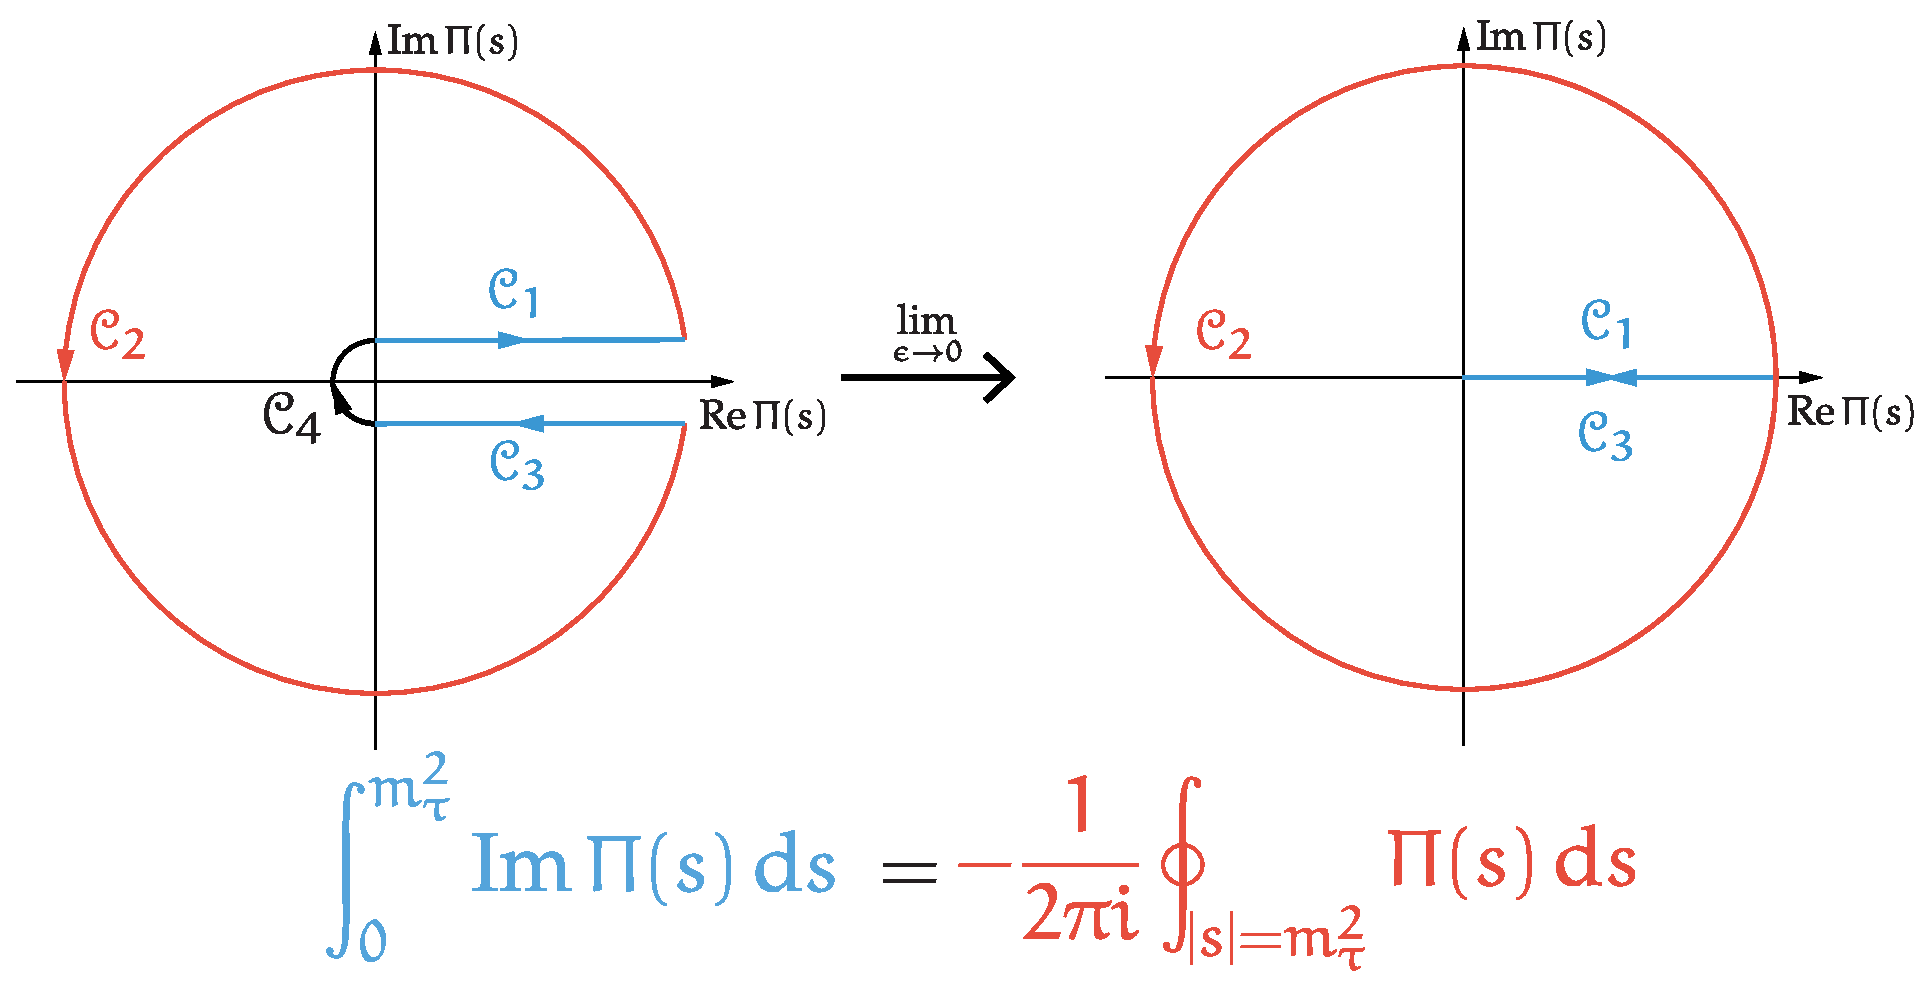
\includegraphics[width=0.9\textwidth]{./images/rTauCauchysTheorem.eps}
\end{frame}
\note[itemize]{
\item We can avoid the positive real axis by making use of Cauchy's theorem 
\item A closed contour integral over an analytic function is zero
\item Thus we get a line integral, which will represent the experimental value,
  equal to a circle contour, with radius of \(m_\tau^2\), which represents the
  theoretical value
\item Applied to the inclusive hadronic tau decay ratio we get equation nine,
  where we also substituted \(\Pi^{(1+0)}\) 
\item Imaginary part of two-point function related to experimental accessible
  spectral function
}

\begin{frame}
  \frametitle{Finite Energy Sum Rules}
  \begin{itemize}
  \item Spectral Function:
    \begin{equation}
      \rho(s) = \frac{1}{\pi} \Ima \Pi(s)
    \end{equation}
    \begin{block}{Integral Moment}
      \begin{equation}
        I_{V/A}^{(\omega)}(s_0) \equiv \frac{12 \pi^2}{s_0} \int_0^{s_0} \dif s \omega\left(\frac{s}{s_0}\right) \rho_{V/A}(s)
        = \frac{6 \pi i}{s_0} \oint_{\abs{s}=s_0} \dif s \omega\left(\frac{s}{s_0}\right) \Pi_{V/A}(s)
      \end{equation}
    \end{block}
    The lhs can be experimentally measured, whereas the rhs has to be
    theoretically calculated.
  \end{itemize}
\end{frame}

\begin{frame}
  \centering
  \vspace{0.3cm}
  \begin{LARGE}
    The Theoretical Computation
  \end{LARGE}
  \begin{equation}
    I^{th}(s_0) \equiv - \frac{1}{2 \pi i s_0} \oint_{\abs{s}=s_0} \dif s \omega\left(\frac{s}{s_0}\right) \Pi_{V/A}(s)
  \end{equation}
\end{frame}

\subsection{Operator Product Expansion}
\begin{frame}
  \frametitle{Operator Product Expansion}
  \begin{itemize}
  \item The two-point function is predicted by the operator product expansion
    \begin{equation}
      \Pi \to \Pi_{OPE}(s) = \sum_D \frac{1}{(-s)^{D/2}} \sum_{dim \mathcal{O} = D} C(-s,\mu)\langle \mathcal{O}(\mu) \rangle
      \equiv \sum_{k=0}^\infty \frac{C_{2k}(s)}{(-s)^k}
    \end{equation}
  \item The term with \(D = 0\) corresponds to the perturbative contribution
  \end{itemize}
\end{frame}
\note[itemize]{
\item The QCD vacuum cannot be solely described perturbatively and we have to
  take non-perturbative effects into account
\item To do so we will describe the two-point function in terms of the operator
  product expansion
\item Here \(A(x)\) and \(B(0)\) are local operators and \(C_n(x)\) is a
  c-number function and \(\mathcal{O}_n(0)\) are higher dimensional operators
\item The OPE separates short distances (high energies/ PT) from long distances
  (NPT)
\item Short distances are given by the Wilson coefficients \(C_n(x-y)\), whereas
  the long distances are given by higher order operators \(\langle \Omega \vert
  \mathcal{O}_n(x) \rangle\).
\item The two-point function can then be written has a series of Wilson
  coefficients multiplied by operators of dimension \(0, 2, \dots\).
\item The Wilson coefficients can be calculated from Feynman diagrams, but the
  higher dimensional contributions have to be taken from NPT tools like lattice
  qcd or from our fits. We will determine values for the dimension six and eight
  operators
\item The dimension zero contribution is the perturbative contribution, whereas
  the higher dimensional contributions are non-perturbative. We will deal with
  the PT contributions first before coming back to the NPT ones. }

\begin{frame}
  \frametitle{Perturbative Contribution}
  \begin{itemize}
  \item In the chiral limit the vector and axial-vector contributions are equal
  \item The renormalisation-scale-invariant Adler function:
    \begin{equation}
      D_{OPE}^{D=0}(s) \equiv -s \frac{\dif}{\dif s} \Pi(s)
      = \frac{1}{4 \pi^2} \sum_{n=0}^\infty a^n(\mu^2) \sum_{k=1}^{n+1} k\, c_{n,k} \log\left( \frac{-s}{\mu^2} \right)^{k-1}
    \end{equation}
    where
    \begin{equation}
      a(\mu^2) \equiv \frac{\alpha(\mu^2)}{\pi}
    \end{equation}
  \item The Adler function only depends on the coefficients \(c_{n,1}\). All
    other \(c_{n,k}\) can be expressed in terms of the \(c_{n,1}\) through the
    RGE.
    \begin{equation}
    c_{0,1} = c_{1,1} = 1, \quad c_{2,1} = 1.63982, \quad c_{3,1} = 6.37101, \quad c_{4,1} = 49.07570, \quad c_{5,1} = 283^*
  \end{equation}
\end{itemize}
\end{frame}
\note[itemize]{
\item It is common to rewrite the two-point function in terms of the Adler
  function.
\item In case of vector correlator the derivative (Adler Function) is a physical
  quantity.
\item Physical quantities are renormalisation scale invariant.
\item The Adler function has different defintions for the \(\Pi^{(1+0)}\) and
  \(\Pi^{(0)}\).
\item Our final expression for the inclusive hadronic tau decay ratio then is
  given in equation 12. }

\begin{frame}
  \frametitle{Perturbative Contribution}
  \begin{itemize}
  \item Perturbative Integral Moment:
    \begin{equation}
      \begin{split}
      I^{th,PT} &\equiv \frac{6 \pi i}{s_0} \oint_{\abs{s}=s_0} \dif s\, \omega\left(\frac{s}{s_0}\right) \Pi_{OPE}^{D=0}(s) \\
      &= \frac{6 \pi i}{s_0} \oint_{\abs{s}=s_0} \frac{\dif s}{s} \omega_D\left(\frac{s}{s_0}\right) D_{OPE}^{D=0}(s) \\
      &= \frac{3 i}{2 \pi s_0} \oint_{\abs{s}=s_0} \frac{\dif s}{s} \omega_D\left(\frac{s}{s_0}\right) \sum_{n=0}^\infty a^n(\mu^2) \sum_{k=1}^{n+1} k\, c_{n,k} \log\left( \frac{-s}{\mu^2} \right)^{k-1}
    \end{split}
  \end{equation}
    where
    \begin{equation}
      \omega_D \equiv \int_0^{s_0} \omega(s^\prime) \dif s
    \end{equation}
  \end{itemize}
\end{frame}


\begin{frame}
  \frametitle{FOPT vs CIPT}
  \begin{itemize}
  \item Perturbative Moment \((x \equiv s/s_0)\)
    \begin{equation}
      I^{th, PT} = \frac{3 i}{2 \pi s_0} \oint_{\abs{x}=1} \frac{\dif x}{x} \omega_D(x) \sum_{n=0}^\infty a^n(\mu^2) \sum_{k=1}^{n+1} k\, c_{n,k} \log\left( \frac{-x s_0}{\mu^2} \right)^{k-1}
    \end{equation}
    \centering
    \begin{tikzpicture}[>=triangle 45,font=\sffamily]
      \node (X) at (0,0) {};
      \node (Y) [below left=1cm and 3cm of X] {};
      \node (Z) [below right=1cm and 3cm of X] {};
      \draw [semithick,->] (X) -- (Y);
      \draw [semithick,->] (X) -- (Z);
    \end{tikzpicture}
    \vspace{-0.2cm}
    \begin{columns}[t]
      \begin{column}{.5\textwidth}
        \centering
        Fixed-Order Perturbation Theory (FOPT)
        \begin{equation*}
          \mu^2 \equiv s_0
        \end{equation*}
        \vspace{-0.5cm}
        - Constant \(a(s_0)\)
      \end{column}
      \begin{column}{.5\textwidth}
        \centering
        Contour-Improved Perturbation Theory (CIPT)
        \begin{equation*}
          \mu^2 \equiv -x s_0
        \end{equation*}
        - Resums the logarithms \\
        - Variable \(a(-x s_0)\)
      \end{column}
    \end{columns}
  \end{itemize}
\end{frame}
\note[itemize]{
\item The general perturbative contribution \(\delta_{pt}\) is defined in
  equation 22, where we plugged in the expanded Adler function in to the tau
  decay ratio and factorised \(12 \pi^2\)
\item Having the freedom to fix \(\mu\) leads to two different treatments of the
  PT contributions
\item FOPT where we fix \(\mu \equiv m_\tau^2\)
\item This leads to a constant \(a_\mu\), so we do not have to run the strong
  coupling. We are left with the integration of the logarithms \(\log(-x)\)
\item On the other hand CIPT fixed \(\mu \equiv -m_\tau^2 x\), which sums up the
  logarithms, but leaves us with a running coupling
\item Both approaches lead to different results }

\begin{frame}
  \frametitle{FOPT vs CIPT}
  \begin{footnotesize}
    Perturbative FOPT and CIPT contributions (\(\alpha(m_\tau^2)=0.34\)):
    \begin{align}
      & \quad\qquad \alpha_s^2 \qquad \alpha_s^2 \qquad \alpha_s^3 \qquad \alpha_s^4 \quad\qquad \alpha_s^5 \nonumber\\
      \delta_{FOPT}^{(0)} &= 0.1082 + 0.0609 + 0.0334 + 0.0174 (+ 0.0088) = 0.2200 (0.2288) \\
      \delta_{CIPT}^{(0)} &= 0.1479 + 0.0297 + 0.0122 + 0.0086 (+ 0.0038) = 0.1984 (0.2021)
    \end{align}

    \vfill

    \begin{center}
      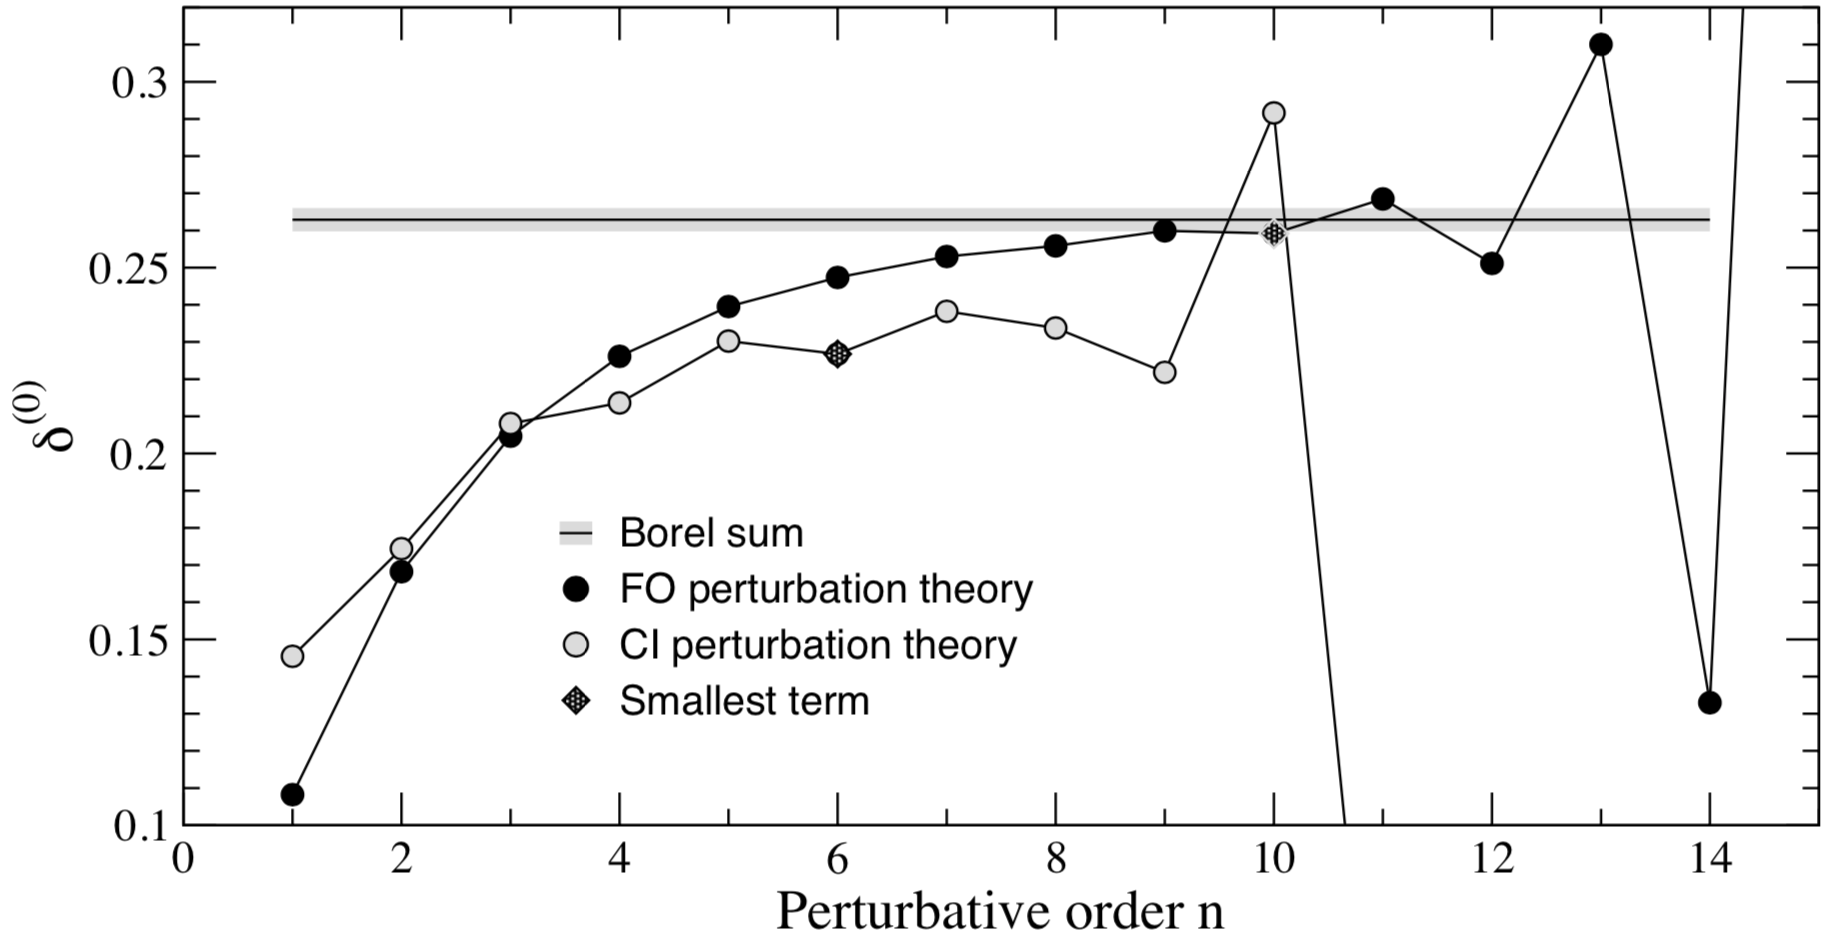
\includegraphics[width=0.7\textwidth]{./images/FOPT_CIPT_contributions.png}
    \end{center}
    \cite{Beneke2008}
  \end{footnotesize}
\end{frame}
\note[itemize]{
\item E.g. here we display the FOPT and CIPT contribution up to fifth order.
\item From the table we can conclude that CIPT converges faster, but has a
  smaller contribution as FOPT, which leads to larger values of \(\alpha_s\)
\item The graph below has been taken from a paper of Beneke and Jamin who
  invested the topic
\item here we see as the black dots the FOPT contribution, as the gray dots the
  CIPT contribution and as a straight line the Borel sum to which we will come
  in a minute to which we will come in a minute to which is used to sum
  asymptotic series like in this case
\item Note that FOPT converges in line with the Borel sum, but CIPT does not
\item We will make the same observation while performing our fits }

\begin{frame}
  \frametitle{Borel Model}
  \begin{itemize}
  \item 
  \item Borel transform and Borel integral:
    \begin{equation}
      A \equiv \int_0^\infty \dif t e^{-t/a} B[A](t) \quad \text{with} \quad B[A](t) = \sum_{n=0}^\infty \frac{a_k}{n!} t^n.
    \end{equation}
  \item Borel model\footcite{Beneke2008}:
    \begin{equation}
      \label{eq:borelModel}
      B[\widehat D](u) = B[\widehat D_1^{UV}](u) + B[\widehat D_2^{IR}](u) + B[\widehat D_3^{IR}](u) + d_0^{PO} + d_1^{PO}u,
    \end{equation}
  \end{itemize}
\end{frame}
\note[itemize]{
\item The Borel summation is a summation method for divergent asymptotic series
  and should give us the best possible sum
\item It consists of the Borel integral and the Borel transform, which we apply
  to the expansion of the Adler function
\item We will follow the notation of \cite{Beneke2008}, which redefined the
  Adler function expansion as \(1 + \hat D(s)\) }

\subsection{Non-Perturbative Contributions}
\begin{frame}
  \frametitle{Non-Perturbative Contributions}
  Operator Product Expansion:
  \begin{equation}
    \Pi_{NPT, V/A}^{OPE}(s) = \sum_{n=2,4,\dots} \frac{C_n \langle \Omega \vert \mathcal{O}_n (x) \vert \Omega \rangle}{(s)^{n/2}}
  \end{equation}

  \vfill

  
  \begin{equation}
    \begin{array}{ll}
      \text{Dimension 0:} & \mathbb{1} \\
      % \text{Dimension 2:} & m_i^2 \\
      \text{Dimension 4:} & :m_i \overline{q} q: \\
                          & :G_a^{\mu\nu}(x) G_{\mu\nu}^a(x): \\
                          % & m_i^4 \\
      \text{Dimension 6:} & :\overline{q} \Gamma q \overline{q} \Gamma q: \\
                          & :\overline{q} \Gamma \frac{\lambda^a}{2} q_\beta(x) \overline{q} \Gamma \frac{\lambda^a}{2} q: \\
                          & :m_i \overline{q} \frac{\lambda^a}{2} \sigma_{\mu\nu} q G^{\mu\nu}_a: \\
                          & :f_{abc} G_a^{\mu\nu} G_b^{\nu\delta} G_c^{\delta\mu}: \\
      \cdots              & \cdots
    \end{array}
  \end{equation}
\end{frame}
\note[itemize]{
  \item Next to the PT contribution we have to implement the NPT contributions
    from the OPE
  \item We can see that the OPE series is suppressed by powers of \(s\) thus we
    can approximate the series by a cutoff
  \item The lowest dimensional operators are given in equation 37
  \item In our analysis we will neglect
    the dimension two contributions as we
    work in the chiral limit and their contributions are proportional to the quark masses
}

\begin{frame}
  \frametitle{Dimension Four Corrections}
  Dimension Four Contributions:
  \begin{equation}
    \left. D_{ij}^{(1+0)}(s) \right\rvert_{D=4} = \frac{1}{s^2} \sum_n \Omega^{(1+0)}(s/\mu^2)a^n,
  \end{equation}
  \begin{small}
    \begin{equation}
      \begin{split}
        &\Omega_n^{(1+0)} (s/\mu^2) \,=\, \frac{1}{6}\langle aGG \rangle p_n^{(1+0)}(s/\mu^2) + \sum_k m_k \langle \overline{q}_k q_k \rangle r_n^{(1+0)}(s/\mu^2) \\
        &\quad+ 2\langle m_i \overline{q}_i q_i + m_j \overline{q}_j q_j \rangle q_n^{(1+0)} (s/\mu^2) \pm \frac{8}{3} \langle m_j \overline{q}_i q_i + m_i \overline{q}_j q_j \rangle t_n^{(1+0)} \\
        &\quad- \frac{3}{\pi^2} (m_i^4 + m_j^4) h_n^{(1+0)} (s/\mu^2) \mp \frac{5}{\pi^2} m_i m_j (m_i^2 + m_j^2) k_n^{(1+0)}(s/\mu^2)\\
        &\quad+ \frac{3}{\pi^2} m_i^2 m_j^2 g_n^{(1+0)}(s/\mu^2) + \sum_k m_k^4
        j_n^{(1+0)}(s/\mu^2) + 2 \sum_{k \neq l} m_k^2 m_l^2 u_n^{(1+0)}(s/\mu^2).
      \end{split}
    \end{equation}
  \end{small}
  \begin{tiny}
    \cite{Pich1999}
  \end{tiny}
\end{frame}
\note[itemize]{
  \item Here is the dimension four OPE contribution, which has been formalised
    in an article by Pich
  \item A lot of coefficient, but what you should take from this slide is the
    Gluon condensate, which we will fit 
}

\begin{frame}
  \frametitle{Dimension Six  and Eight Corrections}
  Higher Dimensional Contributions:
  \begin{equation}
    \begin{split}
      D_{ij,V/A}^{(1+0)} \biggr\rvert_{D=8} = 4 \frac{\rho_{V/A}^{(8)}}{s^4} \\
      D_{ij,V/A}^{(1+0)} \biggr\rvert_{D=10} = 5 \frac{\rho_{V/A}^{(10)}}{s^5} \\
      D_{ij,V/A}^{(1+0)} \biggr\rvert_{D=12} = 6 \frac{\rho_{V/A}^{(12)}}{s^6}
    \end{split} 
  \end{equation}
\end{frame}
\note[itemize]{
  \item Higher order OPE contributions are problematic to parametrise 
  \item Starting from dimension six we will apply the simplest approach possible
    to parametrise the higher dimensional OPE contributions.
  \item We will define a constant \(\rho\) for every dimension, which represents
    the contribution
  \item needs backup slide! why simplest approach
}


\subsection{Duality}
\begin{frame}
  \frametitle{Duality}
  \begin{itemize}
  \item Duality:
    \begin{equation}
      \Pi(s) \to \Pi_{OPE}(s)
    \end{equation}
    
  \item Duality Violations (DV):
    \begin{equation}
      \Delta(s) \equiv \Pi(s) - \Pi_{OPE}(s)
    \end{equation}
    % \begin{equation}
    %   R_{\tau,V/A}^\omega = \frac{N_c}{2} S_{EW} \abs{V_{ud}}^2 (1 + \delta_{pt}^\omega + \delta_{npt}^\omega + \delta_{DV}^\omega)
    % \end{equation}
    \vfill
  \item DV Model:
    \begin{equation}
      \rho_{V/A}^{DV}(s) = e^{-(\delta_{V/A} + \gamma_{V/A}s)} \sin(\alpha_{V/A} + \beta_{V/A}s)
    \end{equation}
    \begin{scriptsize}
      \cite{Boito2011a}
    \end{scriptsize}
  \item DV Contribution:
    \begin{equation}
      D_\omega(s_0) = -12 \pi^2 S_{EW} \abs{V_{ud}}^2 \int_{s_0}^\infty \frac{\dif s}{s_0} \omega(s) \rho_{V/A}^{DV}
    \end{equation}
  \end{itemize}
\end{frame}
\note[itemize]{
  \item We can represent duality as \(\Pi(s) \to \Pi_{OPE}(s)\)
  \item The difference \(\Delta(s)\) defines the duality violating contribution
    to \(\Pi\)
  \item DV can be parametrised via a model
  \item The model has four parameters for the vector and four parameters for the
    axial channel
  \item Too many parameters: e.g. \(\alpha_s, \rho_6, \rho_8\) three parameters
    vs eight!
  \item We will further research the necessity of including DV
}

\subsection{Experiment}

\subsection{Inclusive Hadronic Tau Decay Ratio}
\begin{frame}
  \frametitle{Inclusive Hadronic Tau Decay Ratio}
  \begin{itemize}
  \item Spectral function \(\rho^{(1+0)}(s)\) is a measurable from the inclusive
    hadronic tau decay ratio
    \begin{equation}
      R_\tau = \frac{\Gamma[\tau^- \to \nu_\tau + \text{hadrons}]}{\Gamma[\tau^- \to \nu_\tau e^- \overline{\nu}_{e}]}
    \end{equation}
  \item Inclusive Hadronic Tau Decay Ratio is given by (\(s \equiv -q^2\))
    \begin{scriptsize}
      \begin{equation}
        R_{\tau} = 12 \pi \,\abs{V_{ud}}^2 S_{EW} \int_0^{m_\tau^2} \frac{\dif s}{m_\tau^2} \left( 1 + 2 \frac{s}{m_\tau^2} \right)
        \left[ \left( 1+2\frac{s}{m_\tau^2} \right) \Ima \Pi^{(1)}(s) + \Ima \Pi^{(0)}(s)\right]
      \end{equation}
    \end{scriptsize}
  \end{itemize}
\end{frame}
\note[itemize]{
  \item A central value is the inclusive hadronic tau decay ratio (i.e. all
    decays containing hadrons)
  \item The ratio can be calculated by using the optical theorem 
  \item \(V_{ud}\) is the Cabbibo matrix element, \(S_{EW}\) the electroweak correction
  \item We have to integrate the two-point function from \(0 \to m_\tau^2\)
  \item The two-point function has poles on the positive real axis, on the
    remaining \(s\) plane the two-point function is analytic
  \item \(\Pi^{(0)}\) will be neglected? There is no \(J=0\) vector
    contribution. The \(J=0\) axial-vector contribution is the pion pole. Which
    is missing in the experimental data.
}
\begin{frame}
  \frametitle{ALEPH Data}
  \begin{itemize}
    \item Experimental Spectral Moment:
      \begin{equation}
        \rho^{(1)}_{V/A}(s) = \frac{m_\tau^2}{12 \pi^2 \abs{V_{ud}}^2 S_{EW}} \frac{\mathcal{B}_{V/A}}{\mathcal{B}_e} \frac{\dif N_{V/A}}{N_{V/A}\dif s}
        \frac{1}{\omega_\tau}
      \end{equation}
  \end{itemize}

  \vfill

  \begin{columns}
    \begin{column}{0.5\textwidth}
      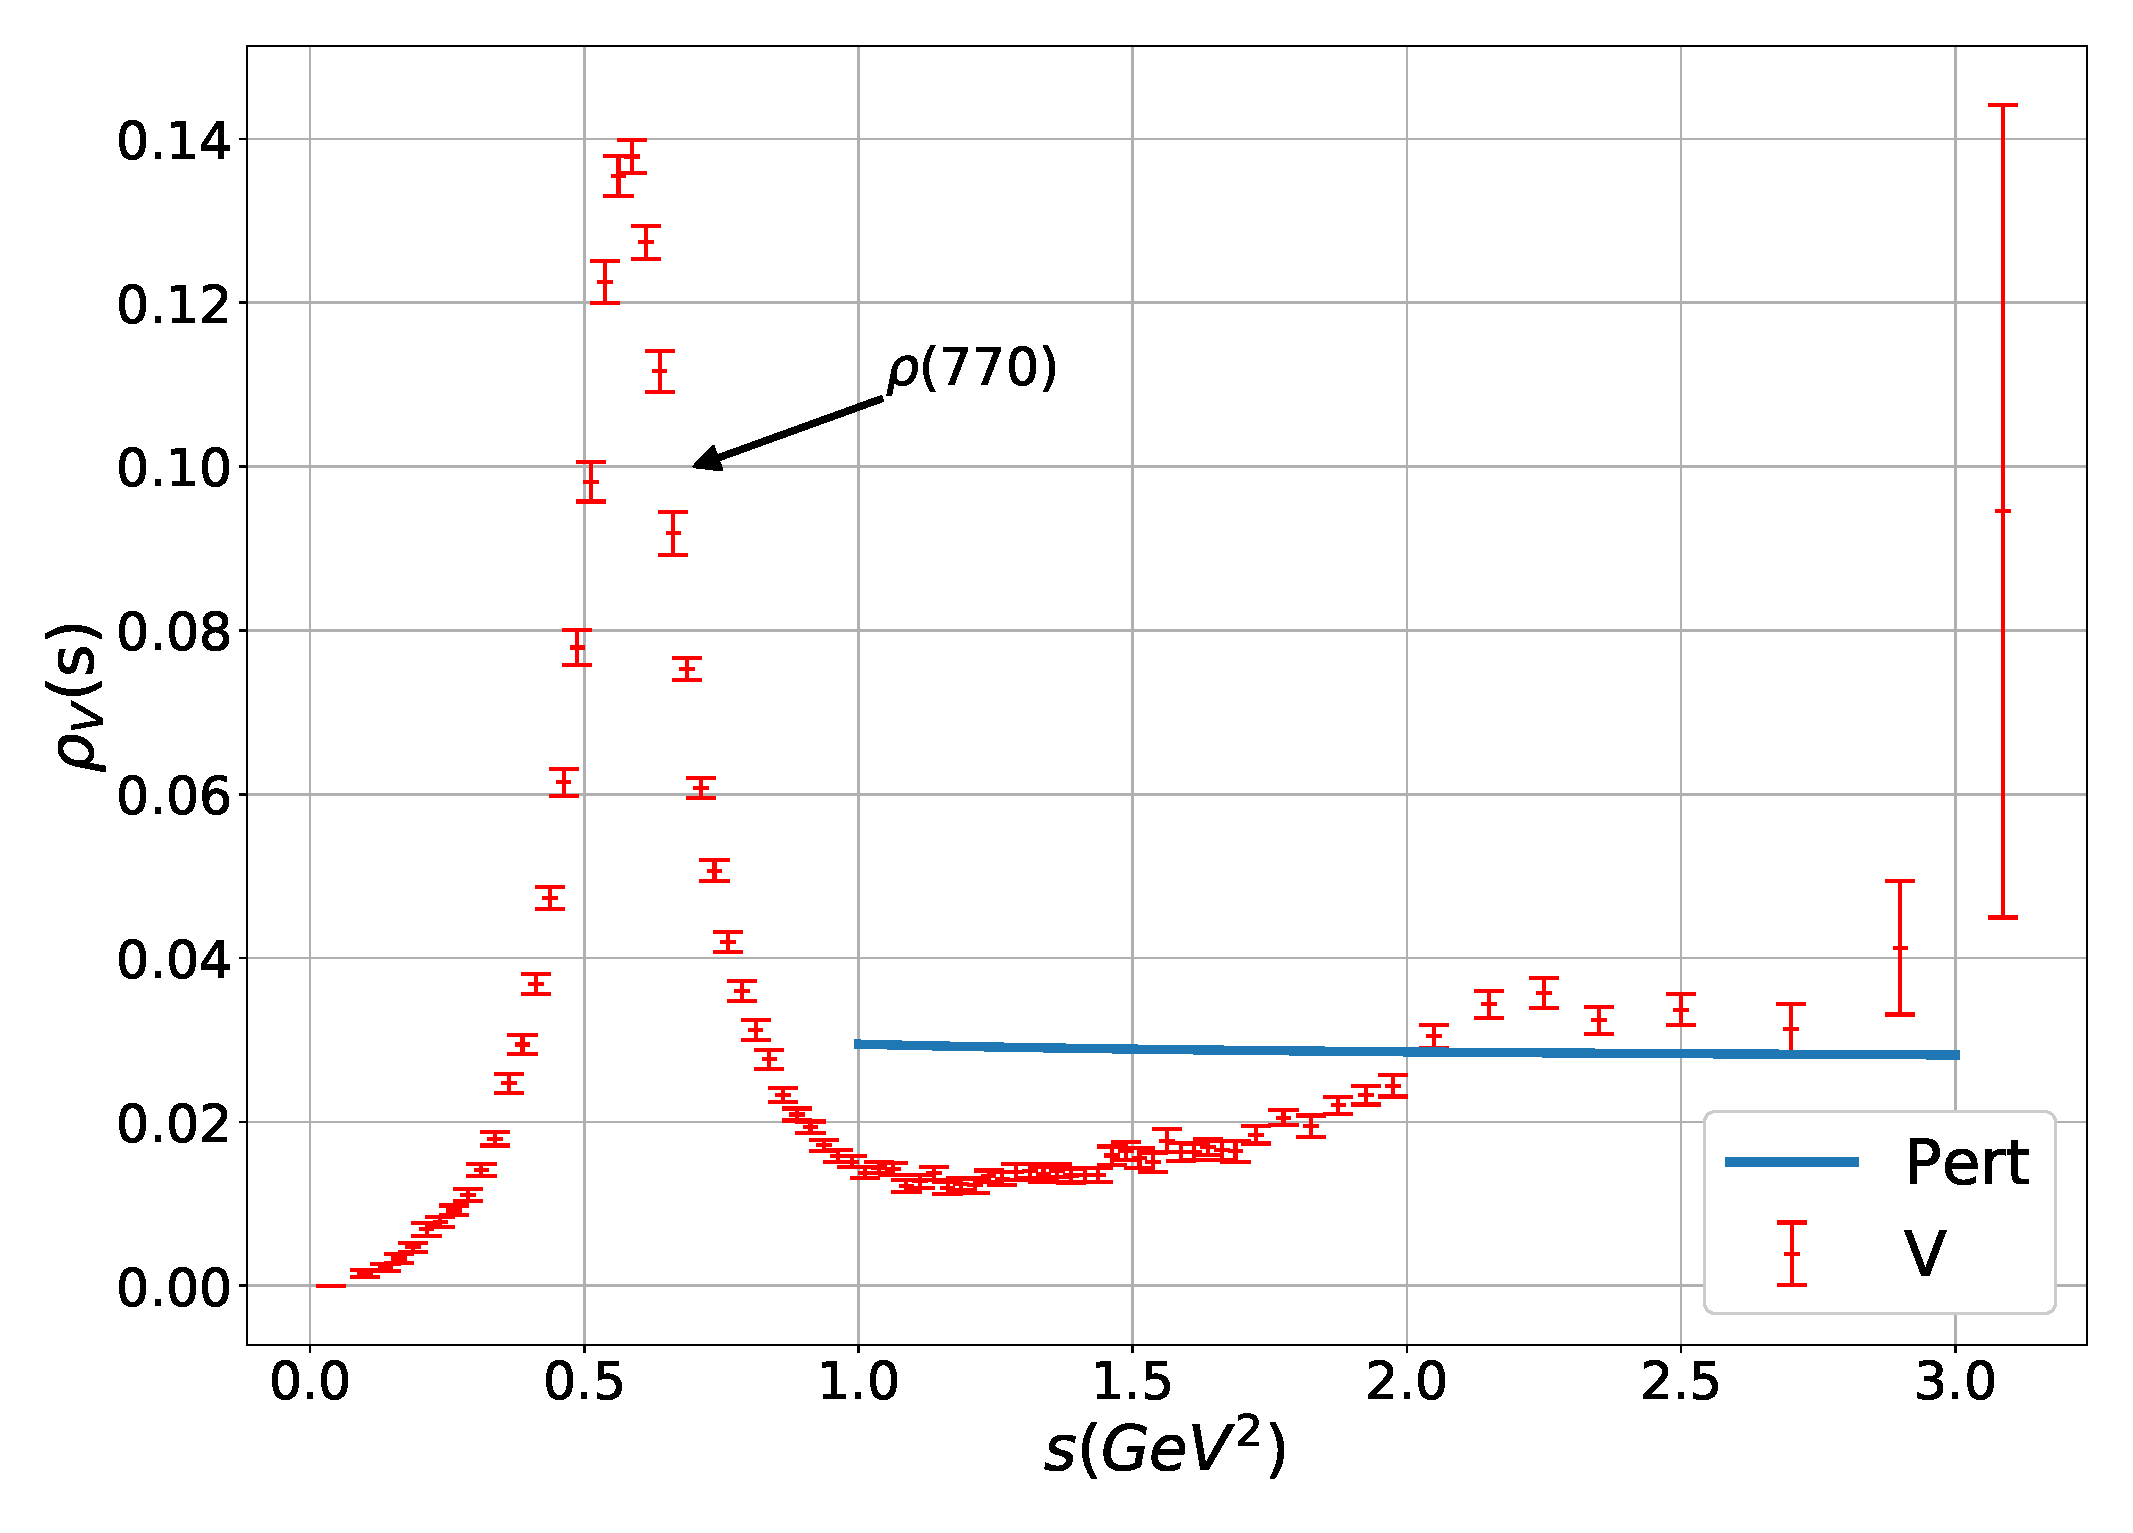
\includegraphics[width=\textwidth]{./images/specFuncAleph_V.eps}
    \end{column}
    \begin{column}{0.5\textwidth}
      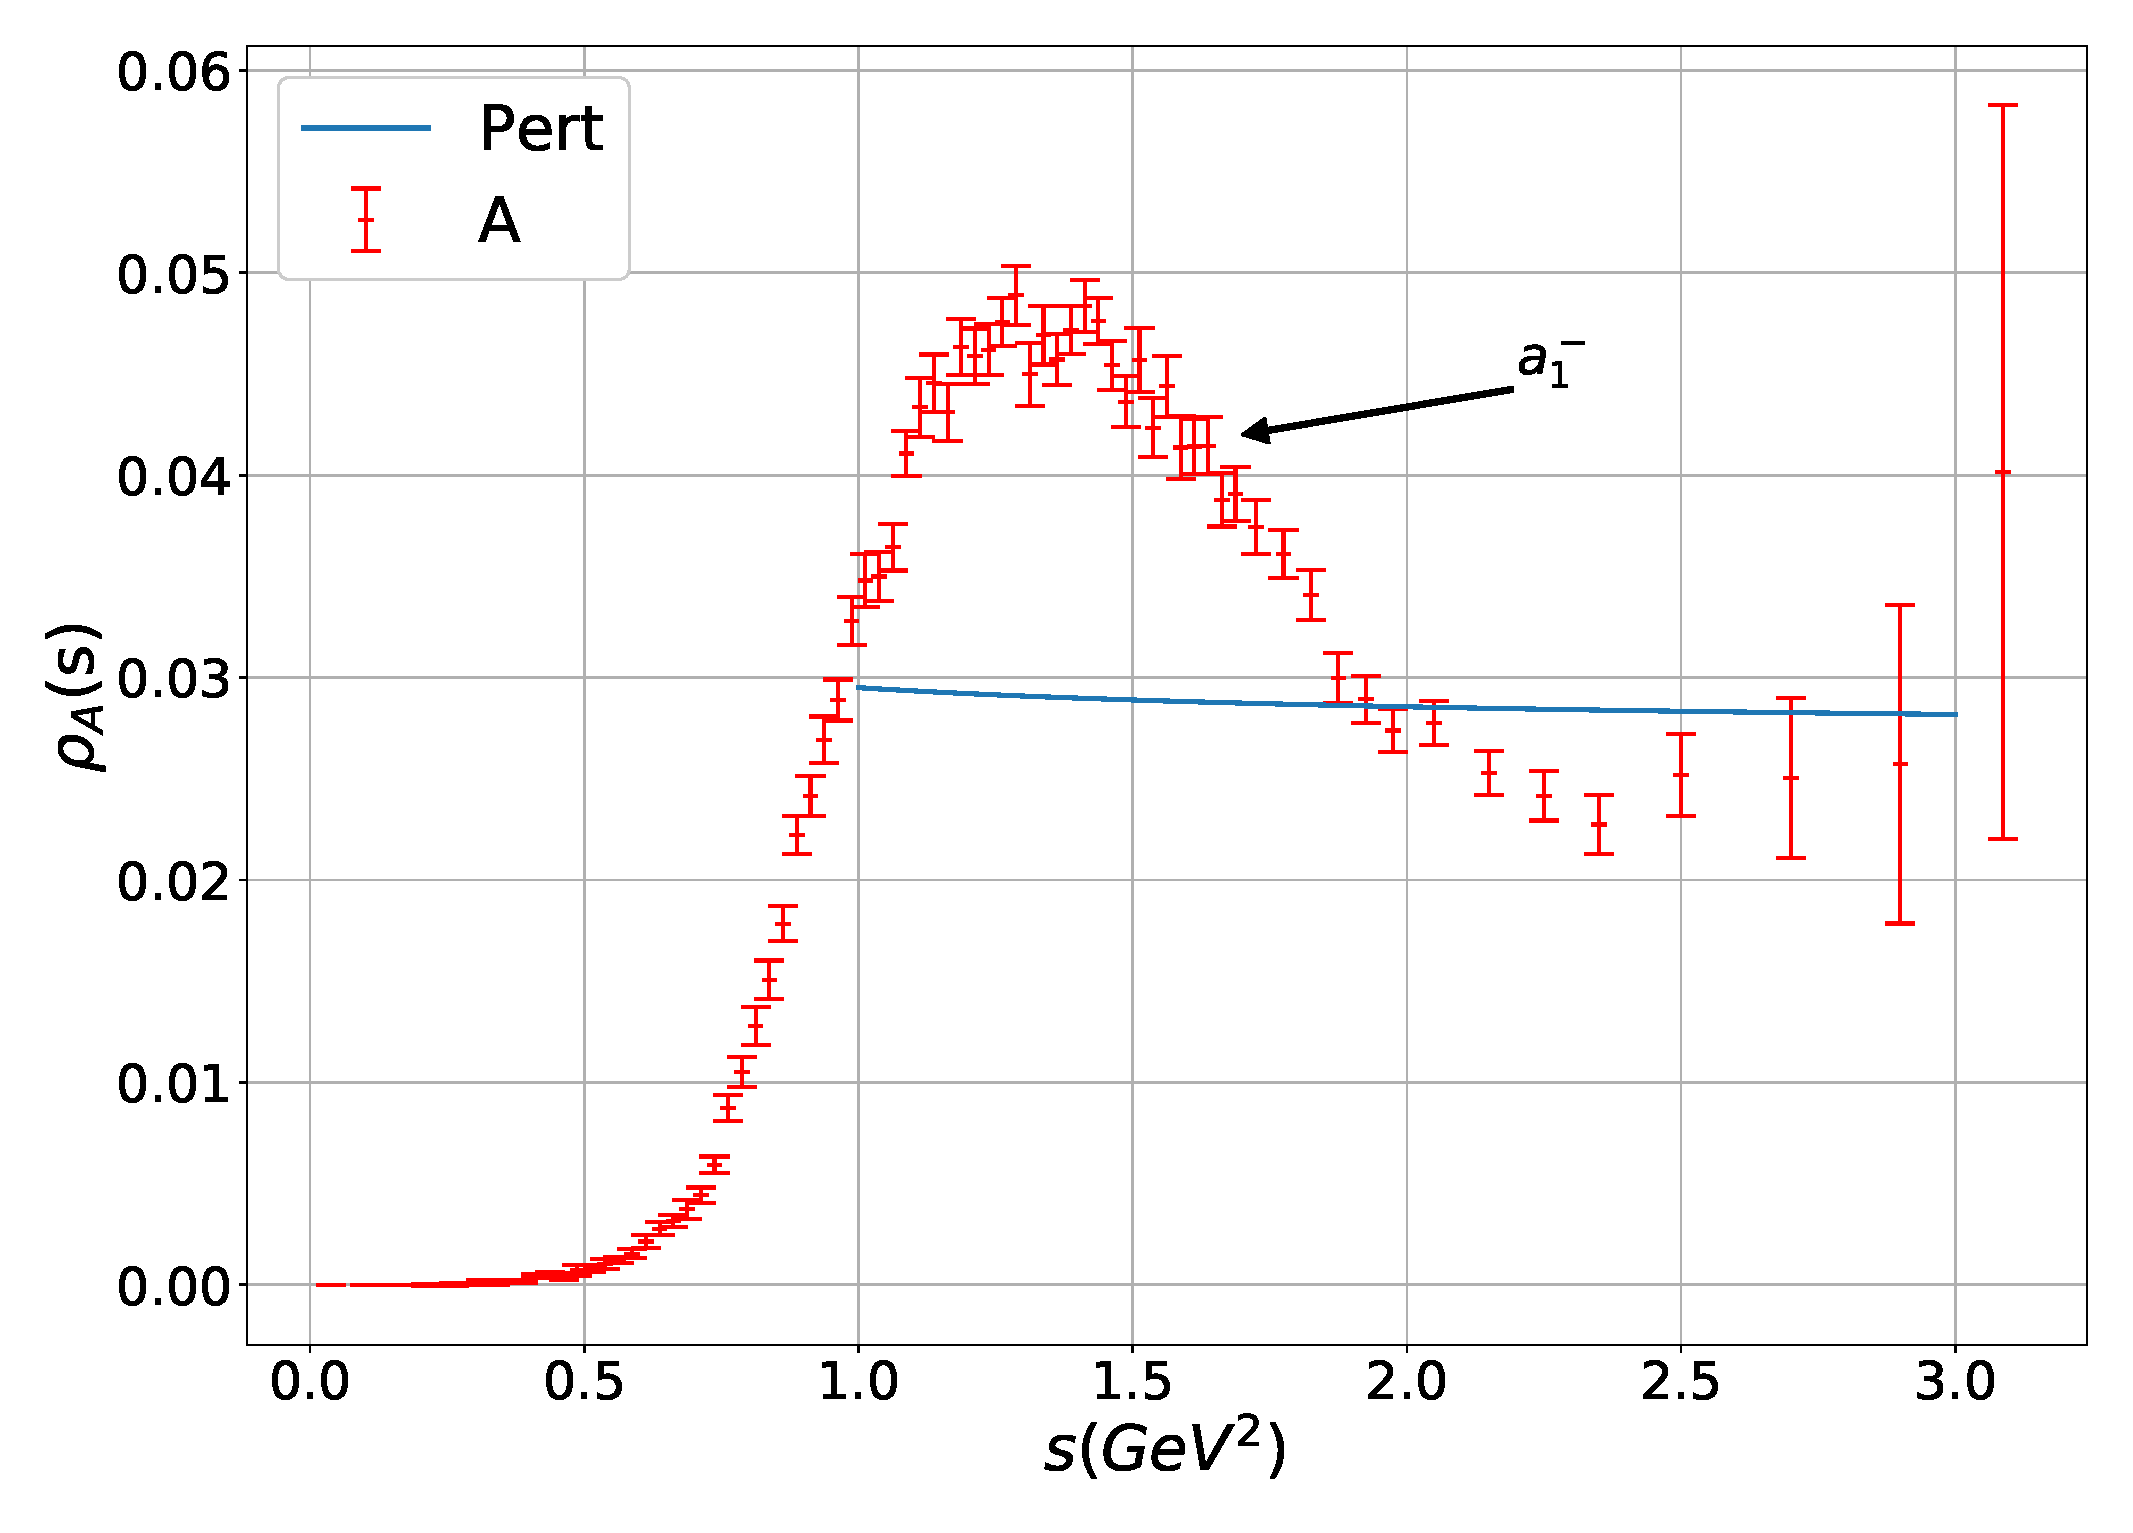
\includegraphics[width=\textwidth]{./images/specFuncAleph_A.eps}
    \end{column}
  \end{columns}
\end{frame}
\note[itemize]{
\item The data we use is given by the ALEPH group
\item ALEPH was a particle detector on the Large Electron-Positron collider in
  the nineties
\item The data is given as a the normalised invariant mass squared distribution
  \(\dif N/ N/ \dif s\) for each channel \(V\), \(A\) and \(V+A\)
\item In the two graphs we see the contribution of the \(V\) channel (left)
  and the \(A\) channel (right)
\item In the vector channel we see the \(\rho(770)\) resonance
\item In the axial channel we see the \(a_1^-\) resonance
\item We also plotted the Perturbative contribution, which cannot reproduce
  the experimental data, especially for lower energies
}

\begin{frame}
  \frametitle{ALEPH Data}
  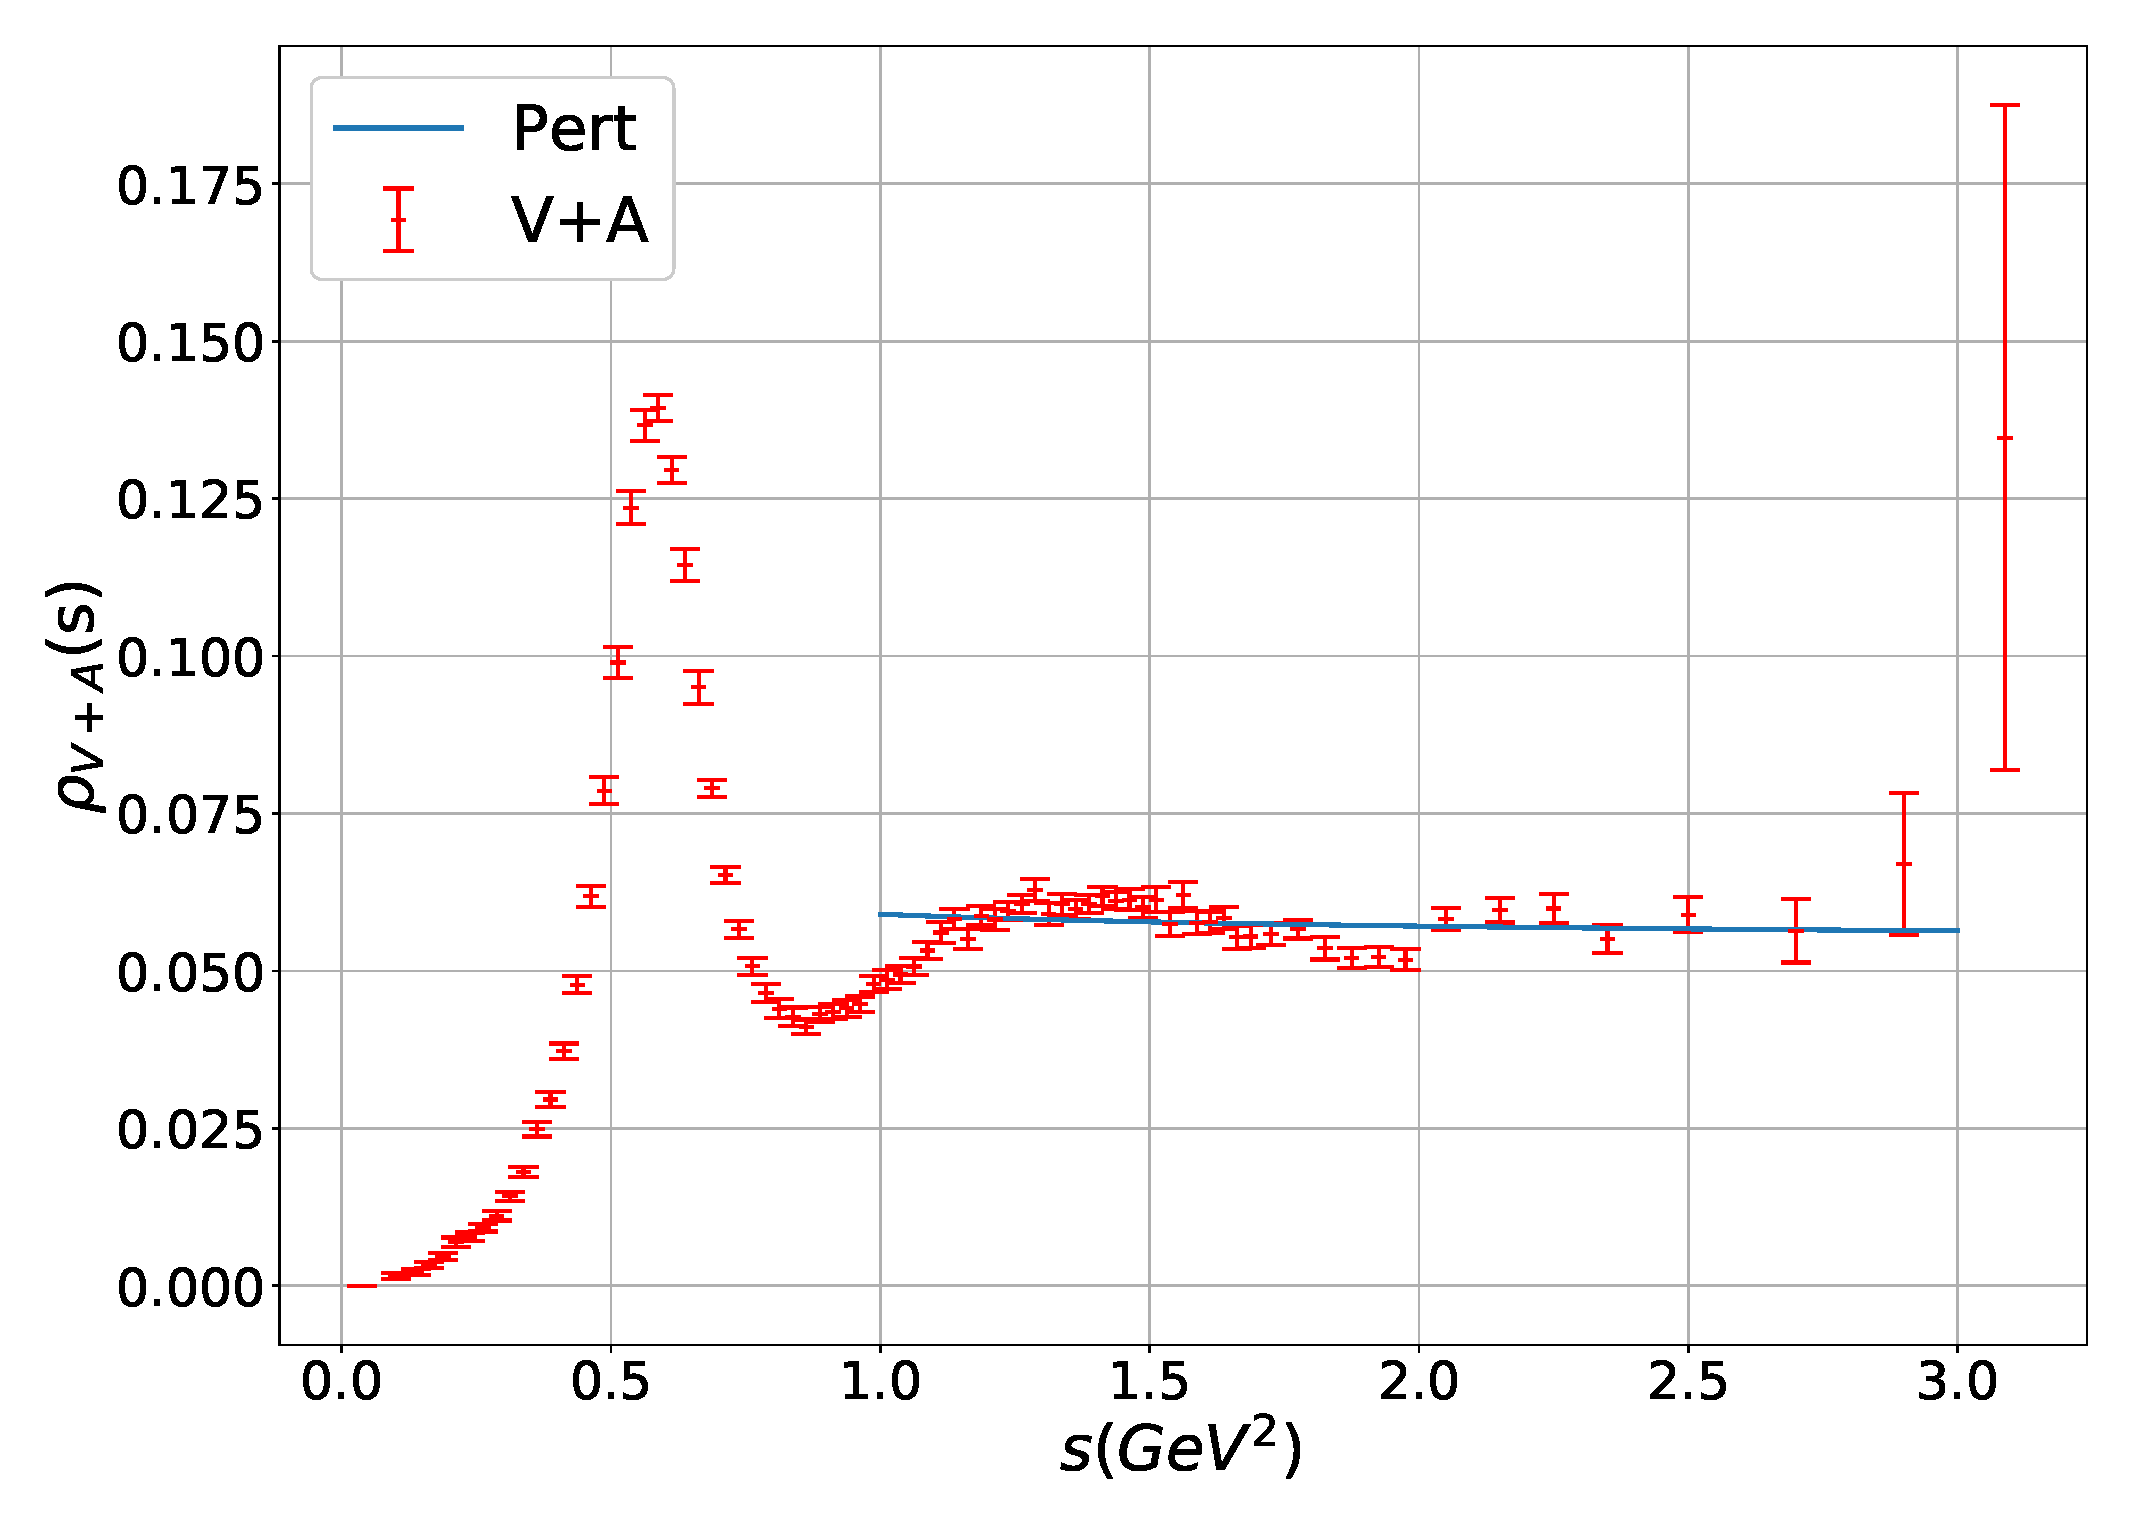
\includegraphics[width=\textwidth]{./images/specFuncAleph_VpA.eps}
\end{frame}
\note[itemize]{
  \item Here we see the experimental spectral function of the \(V+A\) channel
  \item Note that for higher energies the perturbative contribution matches the
    spectral function far better
  \item Also note that we still see a wavy behaviour of the spectral function in
    the data, which is connected to Duality Violations
  \item We assume that in the \(V+A\) channel DV are sufficiently suppressed to
    avoid modelling their contributions
}

\begin{frame}
  \frametitle{Integral Moments}
  \begin{itemize}
    \item Integral Moment:
      \begin{footnotesize}
        \begin{equation}
          I_{V/A}^\omega(s_0) \equiv 12 \pi^2 \int_0^{s_0} \frac{\dif{s}}{s_0} \omega\left( \frac{s}{s_0}\right) \rho^{exp}_{V/A}(s)
          = \frac{3 \pi}{i} \oint_{\abs{s}=s_0} \frac{\dif s}{s_0} \omega\left(\frac{s}{s_0}\right) D^{th}(s) 
        \end{equation}
      \end{footnotesize}
    \item Experimental Moment:
      \begin{equation}
        I_{exp,V/A}^\omega (s_0) = \frac{m_\tau^2}{\mathcal{B}_e s_0}
        \sum_{i=1}^{N(s_0)} \frac{\omega(s_i/s_0)}{\omega_\tau (s_i/s_0)} \sfm2_{V/A}(s_i)
      \end{equation}
  \end{itemize} 
\end{frame}
\note[itemize]{
  \item We defined the so-called integral moments, which we will use to define
    our chi-squared function
  \item the experimental moment is then a sum given by equation 47   
  \item \(\sfm2\) is given in the binned data of the aleph group 
  \item \(\sfm2_{V/A} \equiv B_{V/A} \frac{\dif N_{V/A}}{N_{V/A} \dif s}\)
  \item \(\rho^{(0)}_V\) does not exist
  \item \(\rho^{(0)}_A\) is the pion pole, which is not included in the data?
}

\subsection{Weights}
\begin{frame}
  \frametitle{Weights}
  \begin{itemize}
    \item Weight function:
      \begin{equation}
        \omega(x) \equiv \sum_i a_i x^i
      \end{equation}
    \item E.g.
      \begin{columns}
        \begin{column}{.3\textwidth}
          \begin{itemize}
            \item double pinched
            \item no monomial
            \item D6 and D8
          \end{itemize}
        \end{column}
        \begin{column}{.5\textwidth}
          \begin{equation}
            \begin{split}
              \omega_\tau &\equiv (1 - x)^2(1 + 2x) \\
              &= 1 - 3x^2 + 2x^3
            \end{split}
          \end{equation}
        \end{column}
      \end{columns}
  \end{itemize}
\end{frame}
\note[itemize]{
  \item The weight is an analytic function
  \item Thus we can define it as an arbitrary polynomial
  \item As an example we can take the natural appearing kinetic weight \(\omega_\tau\)
  \item It is double pinched, does not contain a monomial and as we will see has
    active D6 and D8 contributions
}

\begin{frame}
  \frametitle{Pinched Weights}
  \begin{itemize}
    \begin{columns}
      \begin{column}{.5\textwidth}
        \centering
        \item Pinched weight
          \begin{equation}
            \omega(x) = \left( 1 - x \right)^k
          \end{equation}
      \end{column}
      \begin{column}{.5\textwidth}
        \begin{center}
          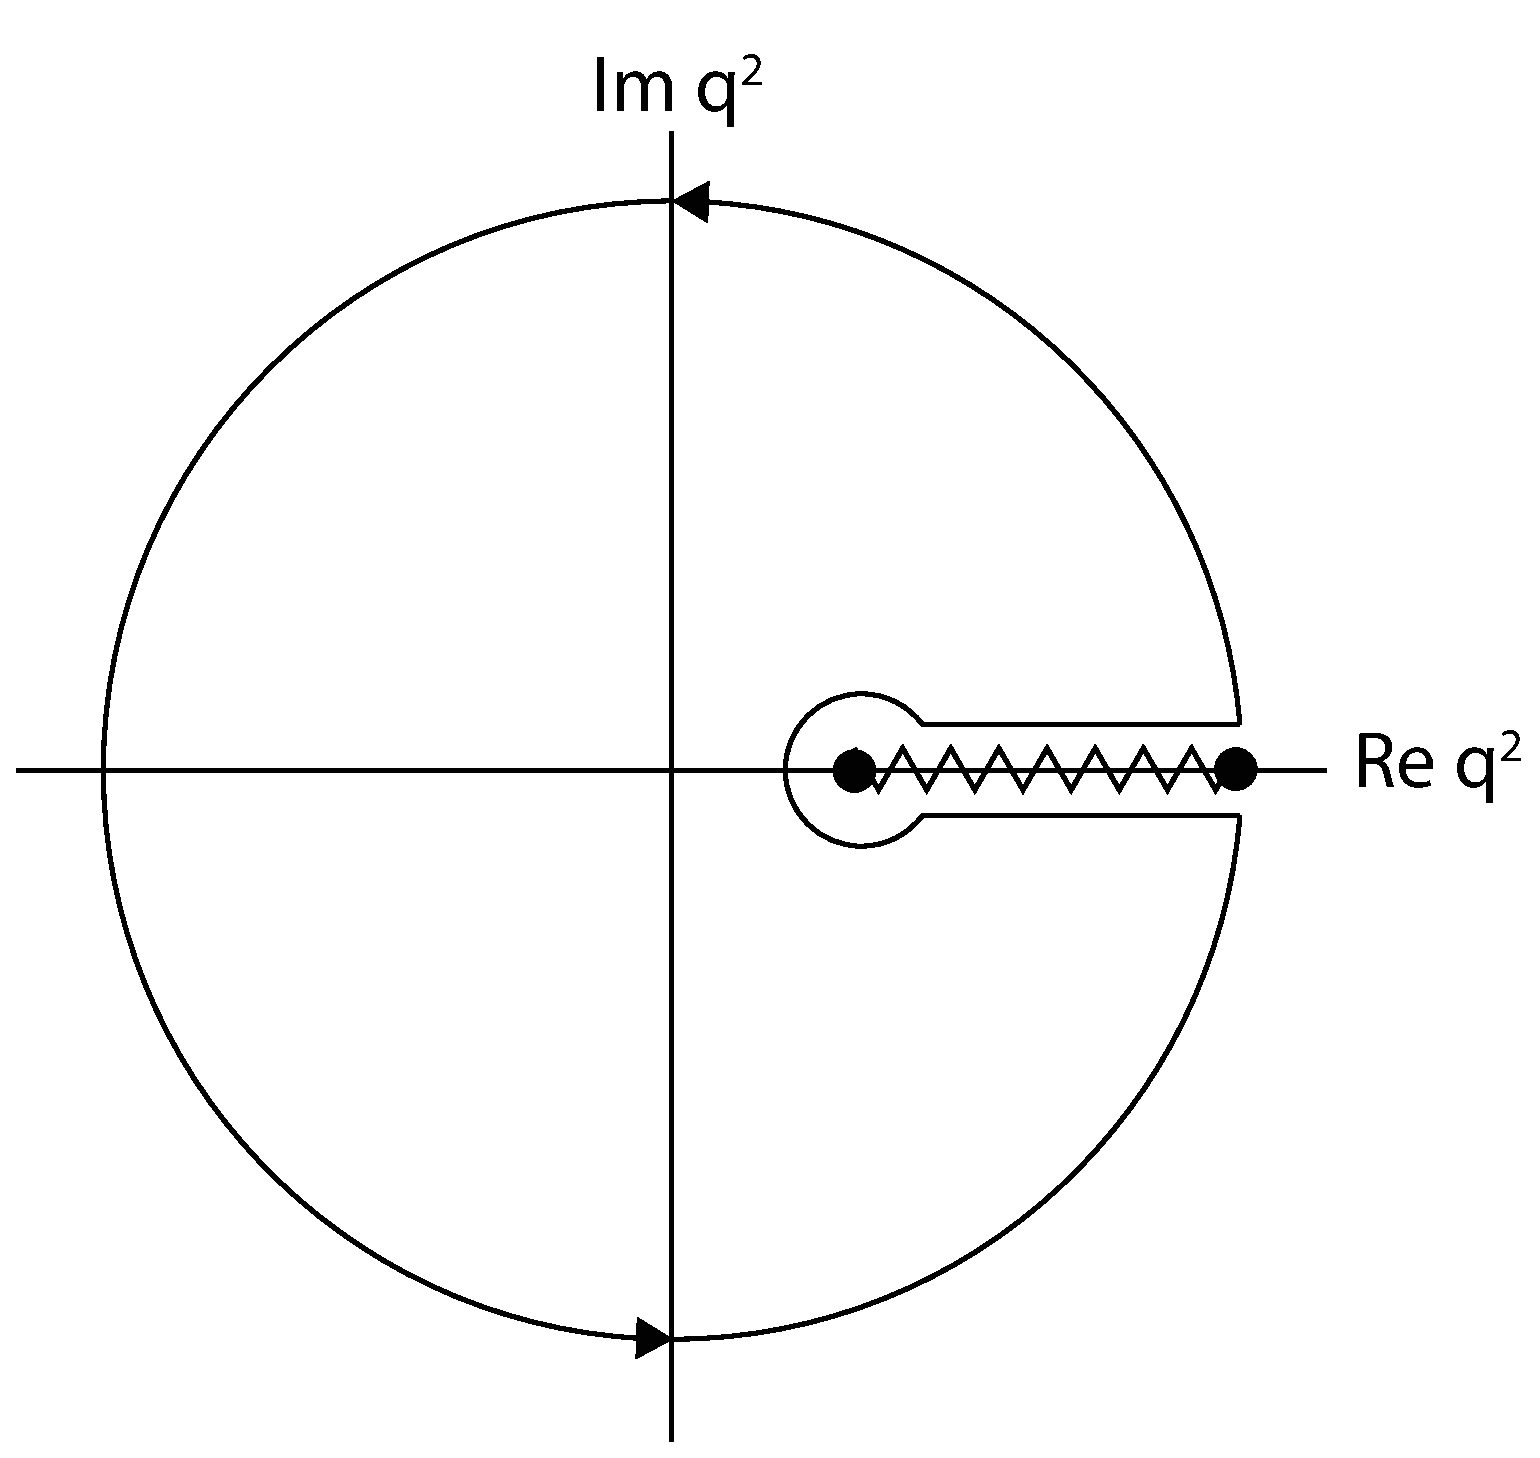
\includegraphics[width=\textwidth]{./images/complexCountour.eps}
        \end{center}
      \end{column}
    \end{columns}
  \end{itemize}
\end{frame}
\note[itemize]{
  \item The theoretical two-point function contains DV close to the positive
    real axis
  \item To suppress DV contributions we introduce pinched weights
  \item The order of the pinching is given by the exponent \(k\) in equation 50
  \item The higher the pinching the fewer the contributions close to the
    positive real axis. This can be seen by plotting the weights. Blue is single
    pinched and decreases linear. Higher pinched weights decrease faster.
  \item Thus implementing a sufficient pinching should avoid DV
}

\begin{frame}
  \frametitle{Weighting OPE Contributions}
  \begin{equation}
    \oint_{C} x^k \dif x = i \int_0^{2\pi}\left(e^{i \theta}\right)^{k+1} \dif \theta
    = \begin{cases} \mbox{\(2 \pi i\)} & \mbox{if } k=-1, \\ \mbox{0} & \mbox{otherwise} \end{cases}.
  \end{equation}
  \begin{equation}
     R(x)\biggr\rvert_{D=0,2,4,\dots} = \oint_{\abs{x}=1} \dif x \, x^{k-D/2} C^{(D)}
  \end{equation}
  \vfill
  Active Dimensions:
  \begin{equation}
    D = 2 (k+1)
  \end{equation}

  \vspace{0.2cm}

  \begin{tabular}{l|ccccccc}
    \toprule
    \textbf{monomial:} & \(x^0\) & \(x^1\) & \(x^2\) & \(x^3\) & \(x^5\) & \(x^6\) & \(x^7\)\\
    \textbf{dimension:} & \(D^{(2)}\) & \(D^{(4)}\) & \(D^{(6)}\) & \(D^{(8)}\) & \(D^{(10)}\) & \(D^{(12)}\) & \(D^{(14)}\)\\
    \bottomrule 
  \end{tabular}
\end{frame}
\note[itemize]{
  \item The weights are also used to ``activate'' different OPE contributions
  \item If we regard a closed contour integral over a \(x^k\), we can see that
    the contour integral is different than zero only if the exponent is equal to \(-1\)
  \item Similarly regarding the integral moment, we see that only certain
    dimensions contribute, while other dimensions are strongly suppressed
  \item Thus the active dimensions are given by \(D = 2(k+1)\)
  \item In the table we can 
  \item (The OPE contributions have logarithmic \(x\) dependence. In general we
    approximated them as constants.)
}


\section{Fits}
\subsection{Strategy}
\begin{frame}
  \frametitle{Chi-Squared}
  \begin{itemize}
    \item Chi-Squared function:
      \begin{equation}
        \chi^2 = (I_i^{exp} - I_i^{th}(\vec \alpha)) C_{ij}^{-1} (I_j^{exp} - I_j^{th}(\vec \alpha))
      \end{equation}
    \item Covariance Matrix:
      \begin{equation}
        C_{ij} = \cov(I_i^{exp}, I_j^{exp})
      \end{equation}

    \item Chi-Squared per Degrees of Freedom:
      \begin{equation}
        \frac{\chi^2}{dof} \approx 1
      \end{equation}
  \end{itemize}
\end{frame}
\note[itemize]{
  \item The chi-squared function is constructed from the theoretical and
    experimental moments
  \item The indices \(i\) and \(j\) represent the dependency of the moments on
    the chosen weight and \(s_0\)
  \item The fits are highly correlated.
  \item The correlation matrix is given with the data.
  \item A good fit is characterised by a \(\chi^2/dof \approx 1\) 
  \item As we have to deal with missing correlations, we will also interpret
    fits with a \(\chi^2/dof\) smaller than 1 as good
}


\begin{frame}
  \frametitle{Parameters and Momenta}
  \begin{columns}
    \begin{column}{.6\textwidth}
      \begin{itemize}
        \item 3 Moments
        \item max three parameters
        \item e.g. \(\alpha_s, \rho_{V/A}^{(6)}, \rho_{V/A}^{(8)}\) (fully determined)
      \end{itemize}
    \end{column}
    \begin{column}{.4\textwidth}
      \begin{tabular}{ccc}
        \toprule
        \# &\multicolumn{2}{c}{3 Moments} \\
        \midrule
        1 & \(s_1\) & \(\omega\) \\
        2 & \(s_2\) & \(\omega\) \\
        3 & \(s_3\) & \(\omega\) \\
        \bottomrule
      \end{tabular}
    \end{column}
  \end{columns}

  \vfill

  \begin{columns}
    \begin{column}{.4\textwidth}
      \centering
      \begin{tabular}{ccc}
        \toprule
        \# &\multicolumn{2}{c}{9 Moments} \\
        \midrule
        1      & \(s_1\) & \(\omega\) \\
        2      & \(s_2\) & \(\omega\) \\
        \vdots & \vdots  & \vdots     \\
        9      & \(s_9\) & \(\omega\) \\
        \bottomrule
      \end{tabular}
    \end{column}
    \begin{column}{.6\textwidth}
      \begin{itemize}
      \item 9 Moments
      \item max nine parameters
      \end{itemize}
    \end{column}
  \end{columns}
\end{frame}
\note[itemize]{
  \item Our ``data points'' are the integral momenta. We will construct multiple
    integral momenta for every fit by varying the number of \(s_0\).
  \item In principle we could also vary the weights, but have not done this
  \item E.g. if we want to fit three parameters as 
}

\begin{frame}
  \frametitle{Strategy}
  \begin{itemize}
    \item Extract \(\alpha_s\)
    \item Probe Duality Violations
    \item FOPT vs CIPT
  \end{itemize}
\end{frame}
\note[itemize]{
  \item To extract \(\alpha_s\) at the \(m_\tau^2\) scale, we perform fits with
    multiple \(s_0\) moments.
  \item We check isolated weights for stability for different \(s_0\) moments
  \item Check stability for different weights and pinchings. If we obtain
    similar weights DV should not be present.
  \item Perform additional fits with the BS. If parameters are similar to FOPT,
    then FOPT should be the preferred framework.
}

\begin{frame}
  \frametitle{Chosen Weights}
  \resizebox{\textwidth}{!}{
    \begin{tabular}{ccccc}
      \toprule
      & Symbol & Term & Expansion & \textsc{ope} Contributions \\
      \midrule
      \parbox[t]{2mm}{\multirow{3}{*}{\rotatebox[origin=c]{90}{\small Pinched}}} & \(\omega_\tau\) & \((1-x)^2(1+2x)\) & \(1 - 3x^2 + 2x^3\) & \(D6, D8\) \\
      & \(\omega_{cube}\) & \((1-x)^3(1+3x)\) & \(1 - 6x^2 + 8x^3 - 3x^4\) & \(D6, D8, D10\) \\
      & \(\omega_{quartic}\) & \((1-x)^4(1+3x)\) & \(1 - 10x^2 + 20x^3 - 15x^4 + 4x^5\) & \(D6, D8, D10, D12\) \\
      \midrule
      \parbox[t]{2mm}{\multirow{3}{*}{\rotatebox[origin=c]{90}{\small Monomial}}} & \(\omega_{M2}\) & \(1 - x^2\) & \(1-x^2\) & \(D6\) \\
      & \(\omega_{M3}\) & \(1 - x^3\) & \(1 - x^3\) & \(D8\) \\
      & \(\omega_{M4}\) & \(1 - x^4\) & \(1 - x^4\) & \(D10\) \\
      \midrule
      \parbox[t]{2mm}{\multirow{4}{*}{\rotatebox[origin=c]{90}{\small Pinched \(+ x\)}}} & \(\omega_{1,0}\) & \((1 - x)\) & \(1 - x\) & \(D4\) \\
      & \(\omega_{2,0}\) & \((1 - x)^2\) & \(1 - 2x + x^2\) & \(D4, D6\) \\
      & \(\omega_{3,0}\) & \((1 - x)^3\) & \(1 - 3x + 3x^2 - x^3\) & \(D4, D6, D8\) \\
      & \(\omega_{4,0}\) & \((1 - x)^4\) & \(1 - 4x + 6x^2 - 4x^3 + x^4\) & \(D4, D6, D8, D10\) \\
      \bottomrule
    \end{tabular}
  }
\end{frame}
\note[itemize]{
  \item To apply the strategy we have to choose several weights
  \item We selected three categories:
    \begin{itemize}
      \item Pinched weights without a monomial term
        \(x\), these are double, triple or quadruple pinched,  
      \item Monomial weights, these weights are single pinched and do not
        contain a monomial term \(x\)
      \item ``Pichs optimal'' weights, these weights are single up to quadruple
        pinched and contain a term monomial in \(x\)
    \end{itemize}
  \item We cannot apply FOPT to weights with a monomial term \(x\)
    \(\Rightarrow\) BS
}

\subsection{Results}
\subsubsection{Pinched Weights without a Monomial term \(x\)}
% \begin{frame}
%   \centering

%   \vspace{0.5cm}

%   \LARGE Pinched Weights
% \end{frame} 
\begin{frame}
  \frametitle{Kinematic Weight: \(\omega_\tau(x) \equiv (1-x)^2(1+2x)\)}
  \centering
  \begin{tabular}{ccccccc}
    \toprule
    & \(s_{min}\) & \#\(s_0\)s & \(\alpha_s(m_\tau^2)\) & \(\rho^{(6)}\) & \(\rho^{(8)}\) & \(\chi^2/dof\)  \\
    \midrule
    \parbox[t]{2mm}{\multirow{1}{*}{\rotatebox[origin=c]{90}{\textsc{bs}}}}
    & 2.200 & 7 & 0.3274(42) & -0.82(21) & -1.08(41) & 0.21 \\
    \midrule
    \parbox[t]{2mm}{\multirow{5}{*}{\rotatebox[origin=c]{90}{\textsc{fopt}}}}
    % 1.500 & 23 & 0.3255(13) & -0.441(10) & -0.2909(34) & 2.00 \\
    % 1.525 & 22 & 0.3255(18) & -0.440(36) & -0.288(45) & 2.10 \\
    % 1.550 & 21 & 0.3265(16) & -0.478(36) & -0.343(50) & 1.81 \\
    % 1.575 & 20 & 0.3269(22) & -0.493(47) & -0.365(58) & 1.86 \\
    % 1.600 & 19 & 0.3272(23) & -0.506(51) & -0.384(64) & 1.94 \\
    % 1.625 & 18 & 0.3284(24) & -0.540(53) & -0.433(68) & 1.788 \\
    % 1.650 & 17 & 0.3283(24) & -0.550(57) & -0.448(74) & 1.90 \\
    % 1.675 & 16 & 0.3284(24) & -0.549(57) & -0.448(79) & 2.04 \\
    % 1.700 & 15 & 0.3281(24) & -0.538(63) & -0.430(87) & 2.19 \\
    % 1.750 & 14 & 0.3291(26) & -0.581(71) & -0.50(10) & 2.21 \\
    % 1.800 & 13 & 0.3293(27) & -0.589(77) & -0.51(11) & 2.43 \\
    % 1.850 & 12 & 0.3281(28) & -0.537(85) & -0.42(13) & 2.5 \\
    % 1.900 & 11 & 0.3272(29) & -0.493(93) & -0.35(15) & 2.65 \\
    % 1.950 & 10 & 0.3232(32) & -0.31(11) & -0.01(18) & 1.13 \\
    % 2.000 & 9 & 0.3234(34) & -0.32(12) & -0.03(21) & 1.31 \\
    & 2.100 & 8 & 0.3256(38) & -0.43(15) & -0.25(28) & 1.30 \\
    & \cellcolor{primary}2.200 & \cellcolor{primary}7 & \cellcolor{primary}0.3308(44) & \cellcolor{primary}-0.72(20) & \cellcolor{primary}-0.85(38) & \cellcolor{primary}0.19 \\
    & 2.300 & 6 & 0.3304(52) & -0.69(25) & -0.80(50) & 0.25 \\
    & 2.400 & 5 & 0.3339(70) & -0.91(39) & -1.29(83) & 0.10 \\
    & 2.600 & 4 & 0.3398(15) & -1.3(1.0) & -2.3(2.5) & 0.01  \\
    \bottomrule
  \end{tabular}
\end{frame}
\note[itemize]{
  \item Starting with the kinematic weight
  \item appears naturally in the inclusive hadronic tau decay ratio
  \item is double pinched \(\Rightarrow\) should suppress DV sufficiently
  \item Has two active OPE dimensions, namely dimension six and eight
  \item Leaves us with three fitting parameters: \(\alpha_s, \rho^{(6)}\) and \(\rho^{(8)}\)
  \item \(s_{min}\) is the smallest invariant mass squared value that is
    included in the fit
  \item One has to imagine that the data is binned and that we construct our
    moments starting from the highest available energy
  \item We then perform fits with an increasing number of \(s_0\)s, including
    more and more bins and thus include lower and lower energies
  \item beginning from \SI{2.2}{\giga\eV^2} the fits get problematic due to the
    appearing resonances
  \item Lets regard the two first lines of the FOPT table, we also applied the
    BS for the best fit
  \item Regarding the \(\chi^2/dof\) we se a jump in its value, which we noted
    for every weight. If we go to too low energies the fits become unreliable,
    which is also notable from the deviating values for the parameters.
  \item We decided to take the fits above, but closest to this threshold to be
    the best fit
  \item  For the fits above the threshold we note a great stability between the
    values obtained for \(\alpha_s\)
  \item We also note too low values for the \(\chi^2/dof\), but believe that
    this caused by missing correlations in the ALEPH data
  \item We also performed the same fit for seven moments applying the BS, which
    is in great agreement
}

\begin{frame}
  \frametitle{Cubic Weight: \(\omega_{cube}(x) \equiv (1-x)^3(1+3x)\)}
  \begin{tabular}{ccccccc}
    \toprule
    \(s_{min}\) & \#\(s_0\)s & \(\alpha_s(m_\tau^2)\) & \(\rho^{(6)}\) & \(\rho^{(8)}\) & \(\rho^{(10)}\) & \(\chi^2/dof\)  \\
    \midrule
    % 1.800 & 13 & 0.3305(37) & -0.493(76) & -0.48(12) & -0.66(20) & 2.99 \\
    % 1.850 & 12 & 0.3303(37) & -0.482(68) & -0.456(100) & -0.62(17) & 3.35 \\
    % 1.900 & 11 & 0.3249(29) & -0.280(20) & -0.088(21) & 0.088(55) & 1.58 \\
    % 1.950 & 10 & 0.3237(26) & -0.232(25) & 0.005(42) & 0.275(93) & 1.67 \\
    2.000 & 9 & 0.3228(26) & -0.196(27) & 0.075(28) & 0.420(56) & 1.96 \\
    \rowcolor{primary}
    2.100 & 8 & 0.3302(40) & -0.52(11) & -0.58(22) & -1.00(45) & 0.43 \\
    2.200 & 7 & 0.3312(43) & -0.56(12) & -0.68(23) & -1.23(50) & 0.55 \\
    2.300 & 6 & 0.336(11) & -0.78(47) & -1.17(98) & -2.38(22) & 0.29 \\
    2.400 & 5 & 0.3330(96) & -0.63(47) & -0.82(10) & -1.51(26) & 0.48 \\
    \bottomrule
  \end{tabular}
\end{frame}
\note[itemize]{
  \item The cubic weight is triple pinched
  \item Has three active OPE contributions, \(D6, D8\), and \(D10\)
  \item Consequently we fitted four paremters
  \item Shows very similar behaviour to the kinematice weight (threshold, low
    \(\chi^2/dof\))
  \item Has also very stable values for \(\alpha_s\)
}

\begin{frame}
  \frametitle{Quartic Weight:  \( \omega_{quartic}(x) \equiv (1-x)^4(1+4x)\)}
  \begin{small}
    \begin{ceqn}
      \begin{equation}
        \begin{split}
          \alpha_s(m_\tau^2) = 0.3290(11), \quad \rho^{(6)}=-0.3030(46), \quad \rho^{(8)}=-0.1874(28), \\
          \rho^{(10)} = 0.3678(45) \quad \text{and} \quad \rho_{(12)}=-0.4071(77).
        \end{split}
      \end{equation}
    \end{ceqn}
  \end{small}
\end{frame}
\note[itemize]{
  \item Too many parameters. Only one fit converged
}

\subsubsection{Comparison}
\begin{frame}
  \frametitle{Comparison}
  \centering \resizebox{\textwidth}{!}{
    \begin{tabular}{cccccccc}
      \toprule
      PT & weight & \(\#s_0\)'s & \(\alpha_s(m_\tau^2)\) & \(\langle aGG \rangle_I\) & \(\rho^{(6)}\) & \(\rho^{(8)}\) & \(\chi^2/dof\)  \\
      \midrule
      \parbox[t]{2mm}{\multirow{4}{*}{\rotatebox[origin=c]{90}{\textsc{fopt}}}}
      & \((1-x)^2(1+2x)\)    & 7 & 0.3308(44) & \(2.1^*\) & -0.72(20) & -0.85(38) & 0.19 \\
      & \((1-x)^3(1+2x)\)    & 8 & 0.3302(40) & \(2.1^*\) & -0.52(11) & -0.58(22) & 0.43 \\ 
      % & \(\omega_{quartic}\) & 2.0 & 0.3290(11) & - & -0.3030(46) &
      % -0.1874(28) & 0.3678(45) & 0.67 \\
      & \(1 - x^2\)          & 7 & 0.3248(52) & \(2.1^*\) & -0.77(22) & \(0^*\)   & 0.38 \\
      & \(1 - x^3\)          & 7 & 0.3214(49) & \(2.1^*\) & \(0^*\)   & -1.01(39) & 0.41 \\
      % & \(\omega_{M4}\) & 2.2 & 0.3203(48) & - & - & - & -1.64(77) & 0.42 \\
      \midrule 
      \parbox[t]{2mm}{\multirow{4}{*}{\rotatebox[origin=c]{90}{\textsc{bs}}}}
      & \((1-x)^2(1 + 2x)\) & 7 & 0.3274(42) & \(2.1^*\)    & -0.82(21)   & -1.08(41) & 0.21 \\
      & \(1 - x\)           & 7 & 0.3246(52) & -0.2262(59)  & \(0^*\)           & \(0^*\)   & 0.38 \\
      & \((1 - x)^2\)       & 7 & 0.3270(54) & -0.0254(61)  & -0.77(21)   & \(0^*\)   & 0.74 \\
      & \((1 - x)^3\)       & 8 & 0.3239(40) & -0.0212(42)  & -0.63(15)   & -0.74(29) & 0.46 \\
      % & \(\omega_X4}\) & 2.1 & 0.3248(21) & -0.02230(47) & -0.6724(63) &
      % -0.834(14) & -1.352(28) & 0.23 \\
      \bottomrule
    \end{tabular}
    }
\end{frame}
\note[itemize]{
  \item Here we gathered the ``best'' fits, which are fits with the highest
    \(\#s_0\)'s, but being above the threshold of unstable fits
  \item We left also out the problematic fourth pinched weights, which include
    too high dimensions of the OPE
  \item We can clearly see that all the values obtained for \(\alpha_s\) are
    very similar
  \item values obtained for \(\rho^{(6)}\) and \(\rho^{(8)}\) are within error boundaries
  \item Even though we used different pinchings, aka different amounts of
    suppression for DV
  \item Note that even a single pinched weights like in the second row of the BS
    we achieve comparable results
  \item Comparing the parameters obtained from FOPT, we also see that they are
    very similar to parameters obtained from the BS
}


\section{Conclusions}
\begin{frame}
  \frametitle{Conclusions}
  \begin{itemize}
  \item We measured \(\alpha_s(m_\tau^2) = 0.3261 \pm 0.0050\), which after
    running yields a value of \(\alpha_s(m_Z^2) = 0.11940 \pm 0.00060 \) and is
    comparable to the world average of \(\alpha_s^{(PDG)}(m_Z^2) = 0.1181 \pm
    0.0011\)\footcite{PDG2018}.
  \item \(\rho^{(6)} = -0.68 \pm 0.2\)
  \item \(\rho^{(8)} = -0.80 \pm 0.38\)
  \item DV not present if using single pinched weights in the V+A channel
  \item FOPT more valid than CIPT
  \end{itemize}
\end{frame}


\begin{frame}
  \centering

  \vspace{0.5cm}

  \LARGE Questions
\end{frame}

\appendix
\begin{frame}
  \frametitle{Constants}
  \centering
  \begin{tabular}{lll}
    \toprule
    Quantity & Value \\
    \midrule
    \(V_{ud}\) & \(0.9742 \pm 0.00021\) \\
    \(S_{EW}\) & \(1.0198 \pm 0.0006\)  \\
    \(B_e\) & \(17.818 \pm 0.023\)      \\
    \(m_\tau\) & \SI{1.77686 \pm 0.12}{\mega\eV} \\
    \(\langle  a GG \rangle_I\) & \SI{0.012}{\giga\eV^2} \\
    \(\langle \anti{q}_{u/d}q_{u/d} \rangle(m_\tau) \) & \SI{-272 \pm 15}{\mega\eV} \\
    \( \anti{s}s / \langle \anti{q}q \rangle \) & 0.8 \pm 0.3 \\
    \bottomrule
  \end{tabular}
\end{frame}
\begin{frame}
  \frametitle{DV-model}
  \begin{equation}
    -\frac{1}{2 \pi i} \oint_{\abs{s}=s_0} \frac{\dif s}{s_0} \omega(s/s_0)
    \Delta_{V/A}(s) = - \int_{s_0}^\infty \frac{\dif s}{s_0} \omega(s/ s_0) \frac{1}{\pi} \Ima \Delta_{V/A}(s)
  \end{equation}
\end{frame}
\begin{frame}
  \frametitle{Pion Pole}
  \begin{ceqn}
    \begin{equation}
      R_{\tau,A}^\omega(s_0, \pi) = 24 \pi^2 \abs{V_{ud}}^2 S_{EW} \frac{f_\pi^2}{s_0}
      \omega \left( \frac{s_\pi}{s_0} \right)
      \left[ 1 - \frac{2 s_\pi}{s_\tau+ 2 s_\pi} \right]
    \end{equation}
  \end{ceqn}
\end{frame}
\subsubsection{Single Pinched Monomial Weights}
\begin{frame}
  \frametitle{\(\omega_{M2}(x) \equiv 1-x^2\)}
  \centering
  \begin{tabular}{ccccc}
    \toprule
    \(s_{min}\) & \#\(s_0\)s & \(\alpha_s(m_\tau^2)\) & \(\rho^{(6)}\) &  \(\chi^2/dof\)  \\
    \midrule
    2.100 & 8 & 0.3179(47) & -0.42(17) & 1.62 \\
    \rowcolor{primary}
    2.200 & 7 & 0.3248(52) & -0.77(22) & 0.38 \\
    2.300 & 6 & 0.3260(60) & -0.85(28) & 0.43 \\
    \bottomrule
  \end{tabular}
\end{frame}
\begin{frame}
  \frametitle{\(\omega_{M3}(x) \equiv 1-x^3\)}
  \centering
  \begin{tabular}{ccccc}
    \toprule
    \(s_{min}\) & \#\(s_0\)s & \(\alpha_s(m_\tau^2)\) & \(\rho^{(8)}\) &  \(\chi^2/dof\)  \\
    \midrule
    % 1.500 & 23 & 0.3160(28) & -0.523(65) & 2.4 \\
    % 1.525 & 22 & 0.3171(28) & -0.578(70) & 2.3 \\
    % 1.550 & 21 & 0.3173(29) & -0.587(76) & 2.42 \\
    % 1.575 & 20 & 0.3187(29) & -0.667(82) & 2.08 \\
    % 1.600 & 19 & 0.3189(30) & -0.679(87) & 2.19 \\
    % 1.625 & 18 & 0.3195(30) & -0.719(94) & 2.24 \\
    % 1.650 & 17 & 0.3205(30) & -0.783(99) & 2.1 \\
    % 1.675 & 16 & 0.3204(31) & -0.77(11) & 2.24 \\
    % 1.700 & 15 & 0.3206(31) & -0.79(11) & 2.39 \\
    % 1.750 & 14 & 0.3202(32) & -0.76(13) & 2.57 \\
    % 1.800 & 13 & 0.3217(33) & -0.88(14) & 2.41 \\
    % 1.850 & 12 & 0.3202(35) & -0.75(16) & 2.4 \\
    % 1.900 & 11 & 0.3202(36) & -0.75(18) & 2.67 \\
    % 1.950 & 10 & 0.3161(38) & -0.40(20) & 1.46 \\
    % 2.000 & 9 & 0.3148(39) & -0.28(22) & 1.47 \\
    2.100 & 8 & 0.3147(44) & -0.27(29) & 1.71 \\
    \rowcolor{primary}
    2.200 & 7  & 0.3214(49) & -1.01(39) & 0.41 \\
    2.300 & 6  & 0.3227(57) & -1.18(54) & 0.46 \\
    2.400 & 5  & 0.3257(67) & -1.58(74) & 0.39 \\
    2.600 & 4  & 0.325(10) & -1.54(1.53) & 0.58 \\
    2.800 & 3  & 0.326(21) & -1.69(4.03) & 1.17 \\
    \bottomrule
  \end{tabular}
\end{frame}
\begin{frame}
  \frametitle{Fourth Power Monomial: \(\omega_{M4}(x) \equiv 1-x^4\)}
  \centering
  \begin{tabular}{ccccc}
    \toprule
    \(s_{min}\) & \#\(s_0\)s & \(\alpha_s(m_\tau^2)\) & \(\rho^{(10)}\) & \(\chi^2/dof\)  \\
    \midrule
    % 1.500 & 23 & 0.3144(27) & -0.572(80) & 2.44 \\
    % 1.525 & 22 & 0.3155(27) & -0.655(90) & 2.34 \\
    % 1.550 & 21 & 0.3157(28) & -0.671(99) & 2.45 \\
    % 1.575 & 20 & 0.3171(28) & -0.80(11) & 2.1 \\
    % 1.600 & 19 & 0.3173(29) & -0.82(12) & 2.21 \\
    % 1.625 & 18 & 0.3180(29) & -0.88(13) & 2.24 \\
    % 1.650 & 17 & 0.3190(30) & -0.98(14) & 2.1 \\
    % 1.675 & 16 & 0.3189(30) & -0.97(15) & 2.24 \\
    % 1.700 & 15 & 0.3192(30) & -1.00(16) & 2.39 \\
    % 1.750 & 14 & 0.3188(32) & -0.96(19) & 2.58 \\
    % 1.800 & 13 & 0.3204(32) & -1.17(21) & 2.39 \\
    % 1.850 & 12 & 0.3190(34) & -0.95(26) & 2.4 \\
    % 1.900 & 11 & 0.3189(35) & -0.94(29) & 2.67 \\
    % 1.950 & 10 & 0.3149(37) & -0.31(34) & 1.47 \\
    % 2.000 & 9 & 0.3137(39) & -0.08(39) & 1.5 \\
    2.100 & 8  & 0.3136(43) & -0.07(54) & 1.75 \\
    \rowcolor{primary}
    2.200 & 7  & 0.3203(48) & -1.64(77) & 0.42 \\
    2.300 & 6  & 0.3216(56) & -2.01(1.13) & 0.47 \\
    2.400 & 5  & 0.3247(66) & -2.98(1.62) & 0.39 \\
    2.600 & 4  & 0.324(10) & -2.86(3.69) & 0.58 \\
    2.800 & 3  & 0.325(20) & -3.43(10.74) & 1.17 \\
    \bottomrule
  \end{tabular}
\end{frame}
\subsubsection{Pinched Weights with a Monomial Term \(x\)}
\begin{frame}
  \frametitle{\(\omega_{1,0} \equiv (1-x)\)}
  \centering
  \begin{tabular}{cccccc}
    \toprule
    & \(s_{min}\) & \#\(s_0\)s & \(\alpha_s(m_\tau^2)\) & \(\langle aGG \rangle_I\) & \(\chi^2/dof\)  \\
    \midrule
    \parbox[t]{2mm}{\multirow{3}{*}{\rotatebox[origin=c]{90}{\textsc{bs}}}}
    & 2.100 & 8 & 0.3176(47) & -0.0134(48) & 1.62 \\
    & \cellcolor{primary}2.200 & \cellcolor{primary}7 & \cellcolor{primary}0.3246(52) & \cellcolor{primary}-0.2262(59) & \cellcolor{primary}0.38 \\
    & 2.300 & 6 & 0.3260(60) & -0.2453(73) & 0.43 \\
    \midrule
    % 1.500 & 23 & 0.3369(26) & -0.0508(43) & 5.7 \\
    % 1.525 & 22 & 0.3376(24) & -0.0514(40) & 5.89 \\
    % 1.550 & 21 & 0.3395(28) & -0.0536(48) & 5.56 \\
    % 1.575 & 20 & 0.3395(28) & -0.0537(47) & 5.87 \\
    % 1.600 & 19 & 0.34047(68) & -0.05458(42) & 5.86 \\
    % 1.625 & 18 & 0.3414(30) & -0.0555(50) & 6.0 \\
    % 1.650 & 17 & 0.3418(30) & -0.0561(51) & 6.35 \\
    % 1.675 & 16 & 0.3430(32) & -0.0571(55) & 6.14 \\
    % 1.700 & 15 & 0.3436(33) & -0.0579(56) & 6.44 \\
    % 1.750 & 14 & 0.3457(36) & -0.0597(64) & 5.72 \\
    % 1.800 & 13 & 0.3462(37) & -0.0603(66) & 6.18 \\
    % 1.850 & 12 & 0.3479(43) & -0.0613(76) & 5.02 \\
    % 1.900 & 11 & 0.3489(46) & -0.0622(82) & 5.06 \\
    % 1.950 & 10 & 0.3528(65) & -0.067(12) & 1.69 \\
    % 2.000 & 9 & 0.3560(93) & -0.071(18) & 0.98 \\
    \parbox[t]{2mm}{\multirow{3}{*}{\rotatebox[origin=c]{90}{\textsc{fopt}}}}
    & 2.100 & 8  & 0.357(12) & -0.072(23) & 0.95 \\
    & 2.200 & 7 &  0.3593(97) & -0.079(19) & 0.2 \\
    & 2.300 & 6 & 0.3589(99) & -0.078(20) & 0.24 \\
    % 2.400 & 5 & 0.360(10) & -0.080(21) & 0.28 \\
    % 2.600 & 4 & 0.359(13) & -0.078(26) & 0.41 \\
    % 2.800 & 3 & 0.375(26) & -0.114(62) & 0.1 \\
    \bottomrule
  \end{tabular}
\end{frame}
\begin{frame}
  \frametitle{\(\omega_{2,0} \equiv (1-x)^2\)}
  \centering
  \begin{tabular}{ccccccc}
    \toprule
    & \(s_{min}\) & \#\(s_0\)s & \(\alpha_s(m_\tau^2)\) & \(\langle aGG \rangle_I\) & \(\rho^{(6)}\) & \(\chi^2/dof\)  \\
    \midrule
    % 1.500 & 23 & 0.3276(13) & -0.0077(10) & 0.330(35) & 2.62 \\
    % 1.525 & 22 & 0.3278(14) & -0.0078(10) & 0.330(38) & 2.75 \\
    % 1.550 & 21 & 0.3299(16) & -0.0092(12) & 0.333(37) & 2.31 \\
    % 1.575 & 20 & 0.3308(25) & -0.0098(13) & 0.334(47) & 2.32 \\
    % 1.600 & 19 & 0.3317(28) & -0.0105(14) & 0.335(54) & 2.38 \\

    % 1.650 & 17 & 0.3345(34) & -0.0124(17) & 0.342(62) & 2.15 \\
    % 1.675 & 16 & 0.3349(25) & -0.0127(15) & 0.342(51) & 2.28 \\
    % 1.700 & 15 & 0.3348(33) & -0.0126(18) & 0.342(58) & 2.47 \\
    % 1.750 & 14 & 0.3372(43) & -0.0145(23) & 0.341(71) & 2.34 \\
    % 1.800 & 13 & 0.3378(31) & -0.0149(20) & 0.339(58) & 2.54 \\
    % 1.850 & 12 & 0.3365(38) & -0.0138(25) & 0.346(60) & 2.72 \\
    % 1.900 & 11 & 0.3355(40) & -0.0128(28) & 0.354(59) & 2.97 \\
    % 1.950 & 10 & 0.3296(47) & -0.0073(34) & 0.418(58) & 1.57 \\
    % 2.000 & 9 & 0.3299(50) & -0.0076(39) & 0.414(64) & 1.83 \\
    % 2.100 & 8 & 0.3331(54) & -0.0108(45) & 0.361(76) & 1.9 \\

    \parbox[t]{2mm}{\multirow{3}{*}{\rotatebox[origin=c]{90}{\textsc{bs}}}}
    & 2.100 & 8 & 0.3207(48) & -0.0170(50) & -0.45(17) & 1.90 \\
    & \cellcolor{primary}2.200 & \cellcolor{primary}7 & \cellcolor{primary}0.3270(54) & \cellcolor{primary}-0.0254(61) & \cellcolor{primary}-0.77(21) & \cellcolor{primary}0.74 \\
    & 2.300 & 6 & 0.3253(63) & -0.0232(75) & -0.69(27) & 0.9  \\
    \midrule
    \parbox[t]{2mm}{\multirow{3}{*}{\rotatebox[origin=c]{90}{\textsc{fopt}}}} & 2.100 & 8 & 0.3331(54) & -0.0108(45) & 0.361(76) & 1.9 \\
    & 2.200 & 7  & 0.3401(57) & -0.0185(52) & 0.220(88) & 0.73 \\
    & 2.300 & 6  & 0.3383(68) & -0.0165(67) & 0.26(12) & 0.89 \\
    % & 2.400 & 5 & 0.3450(93) & -0.0243(99) & 0.10(17) & 0.71 \\
    % & 2.600 & 4 & 0.337(16) & -0.014(18) & 0.36(45) & 0.98 \\
    \bottomrule
  \end{tabular}
\end{frame}
\begin{frame}
  \frametitle{\(\omega_{3,0} \equiv (1-x)^3\)}
  \begin{adjustbox}{max width=\textwidth}
    \begin{tabular}{cccccccc}
      \toprule
      & \(s_{min}\) & \#\(s_0\)s & \(\alpha_s(m_\tau^2)\) & \(\langle aGG \rangle_I\) & \(\rho^{(6)}\) & \(\rho^{(8)}\) & \(\chi^2/dof\)  \\
      \midrule
      \parbox[t]{2mm}{\multirow{3}{*}{\rotatebox[origin=c]{90}{\textsc{bs}}}}
      & 2.000 & 9 & 0.3169(20) & -0.0123(34) & -0.29(12) & -0.05(24) & 2.0 \\
      & \cellcolor{primary}2.100 & \cellcolor{primary}8 & \cellcolor{primary}0.3239(40) & \cellcolor{primary}-0.0212(42) & \cellcolor{primary}-0.63(15) & \cellcolor{primary}-0.74(29) & \cellcolor{primary}0.46 \\
      & \cellcolor{primary}2.200 & \cellcolor{primary}7 & \cellcolor{primary}0.3251(17) & \cellcolor{primary}-0.02283(56) & \cellcolor{primary}-0.689(12) & \cellcolor{primary}-0.879(33) & \cellcolor{primary}0.56 \\
      \midrule
      \parbox[t]{2mm}{\multirow{3}{*}{\rotatebox[origin=c]{90}{\textsc{fopt}}}}
      % & 1.900 & 11 & 0.34281(92) & -0.01473(73) & -0.103(22) & -0.534(46) & 1.52
      % \\
      % & 1.950 & 10 & 0.34154(99) & -0.01304(61) & -0.050(17) & -0.389(44) & 1.42
      % \\
      & 2.000 & 9  & 0.33985(81) & -0.01124(43) & 0.002(10) & -0.242(26) & 1.59 \\
      & 2.100 & 8  & 0.3480(47) & -0.0201(36) & -0.264(89) & -1.03(28) & 0.31 \\
      & 2.200 & 7  & 0.3483(23) & -0.0204(41) & -0.27(15) & -1.05(40) & 0.41 \\
      % & 2.300 & 6 & 0.3522(64) & -0.0249(62) & -0.42(18) & -1.51(57) & 0.29 \\
      % & 2.400 & 5 & 0.3480(89) & -0.0199(100) & -0.25(33) & -0.96(10) & 0.39 \\
      \bottomrule
    \end{tabular}
  \end{adjustbox}
\end{frame}
\begin{frame}
  \frametitle{\(\omega_{4,0} \equiv (1-x)^4\)}
  \begin{adjustbox}{max width=\textwidth}
    \begin{tabular}{ccccccccc}
      \toprule
      & \(s_{min}\) & \#\(s_0\)s & \(\alpha_s(m_\tau^2)\) & \(aGGInv\) & \(\rho^{(6)}\) & \(\rho^{(8)}\) & \(\rho^{(10)}\) & \(\chi^2/dof\)  \\
      \midrule
      \parbox[t]{2mm}{\multirow{3}{*}{\rotatebox[origin=c]{90}{\textsc{bs}}}}
      & 1.950 & 10 & 0.31711(67) & -0.012432(24) & -0.30013(73) & -0.06785(16) & 0.26104(50) & 1.09 \\
      & \cellcolor{primary}2.000 & \cellcolor{primary}9 & \cellcolor{primary}0.3206(24) & \cellcolor{primary}-0.0167(14) & \cellcolor{primary}-0.455(38) & \cellcolor{primary}-0.373(67) & \cellcolor{primary}-0.36(14) & \cellcolor{primary}0.83 \\
      & \cellcolor{primary}2.100 & \cellcolor{primary}8 & \cellcolor{primary}0.3248(21) & \cellcolor{primary}-0.02230(47) & \cellcolor{primary}-0.6724(63) & \cellcolor{primary}-0.834(14) & \cellcolor{primary}-1.352(28) & \cellcolor{primary}0.23 \\
      \midrule
      \parbox[t]{2mm}{\multirow{2}{*}{\rotatebox[origin=c]{90}{\textsc{fopt}}}}
      & 1.950 & 10 & 0.3416(14) & -0.01306(83) & -0.050(22) & -0.390(59) & -0.50(19) & 1.71 \\
      & 2.100 & 8 & 0.3480(25) & -0.0201(27) & -0.264(91) & -1.02(23) & -339.00(20) & 0.41 \\
      \bottomrule
    \end{tabular}
  \end{adjustbox}
\end{frame}





\begin{frame}
  \printbibliography
\end{frame}

\end{document}

% LocalWords:  eps
